% !TEX root = main.tex
% !TEX encoding = UTF-8

% !TEX encoding = UTF-8
%======================================================================
% 1. LỚP TÀI LIỆU VÀ ENCODING
%======================================================================
\documentclass[12pt, a4paper, oneside]{report}

% Hỗ trợ gõ tiếng Việt và hiển thị đúng
\usepackage[utf8]{vietnam}
\usepackage[T5]{fontenc}
\usepackage{textcomp}

% Thiết lập font chữ Times New Roman hoặc tương đương
\usepackage{mathptmx} 

%======================================================================
% 2. CANH LỀ VÀ LAYOUT TRANG
%======================================================================
\usepackage[top=3cm, bottom=3cm, left=3.5cm, right=2cm, heightrounded, headheight=15pt]{geometry}

\usepackage{fancyhdr}
\pagestyle{fancy}
\fancyhf{} 
\lhead{\footnotesize\leftmark} 
\cfoot{\footnotesize\thepage} 
\renewcommand{\headrulewidth}{0.4pt}
\renewcommand{\footrulewidth}{0.4pt}

\usepackage{setspace}
\onehalfspacing
\usepackage{indentfirst}

%======================================================================
% 3. CÁC GÓI TOÁN HỌC
%======================================================================
\usepackage{amsmath}    
\usepackage{amssymb}    
\usepackage{amsthm}     
\usepackage{latexsym}   
\usepackage{amsbsy}     
\numberwithin{equation}{chapter} 

\newtheorem{definition}{Định nghĩa}[chapter]
\newtheorem{theorem}{Định lý}[chapter]
\newtheorem{corollary}{Hệ quả}[chapter]
\newtheorem{lemma}{Bổ đề}[chapter]

%======================================================================
% 4. HÌNH ẢNH, MÀU SẮC & GIAO DIỆN
%======================================================================
\usepackage{graphicx}   
\usepackage{svg}        
\usepackage[table, svgnames, xcdraw]{xcolor} % Gộp tất cả option màu vào 1 dòng
\usepackage{tikz}       
\graphicspath{{./images/}} 

\usepackage[labelfont=bf, font=small, skip=5pt]{caption}
\usepackage{subcaption} 
\usepackage{float}      % Hỗ trợ lệnh [H] cho ảnh/bảng
\usepackage{framed}     % [RẤT QUAN TRỌNG] Hỗ trợ môi trường leftbar
\usepackage[most]{tcolorbox}
\usepackage{pdfpages}

\counterwithin{figure}{chapter} 
\counterwithin{table}{chapter}  

%======================================================================
% 5. BẢNG BIỂU
%======================================================================
\usepackage{booktabs}   
\usepackage{tabularx}   
\usepackage{multirow}   
\usepackage{longtable}  
\usepackage{array}      

%======================================================================
% 6. ĐỊNH DẠNG CODE & LIST
%======================================================================
\usepackage{verbatim}
\usepackage{enumitem}

% Sử dụng minted (Lưu ý: Yêu cầu -shell-escape khi biên dịch)
\usepackage{minted}
\setminted{
    frame=lines,      
    framesep=2mm,     
    baselinestretch=1.2,
    fontsize=\small,  
    linenos           
}

% Định dạng lại tiêu đề chương, mục
\usepackage{titlesec}
\titleformat{\chapter}[display]
  {\normalfont\huge\bfseries\centering}{\chaptertitlename\ \thechapter}{20pt}{\Huge}
\titlespacing*{\chapter}{0pt}{50pt}{40pt}

%======================================================================
% 7. TÀI LIỆU THAM KHẢO VÀ HYPERLINK (PHẢI NẰM CUỐI CÙNG)
%======================================================================
\usepackage{csquotes}
\usepackage[
    backend=biber,      
    style=numeric,      
    sorting=none,       
    giveninits=true     
]{biblatex}
\addbibresource{bibliography.bib}

\usepackage{url}        
\usepackage[
    colorlinks=true,      
    linkcolor=black,      
    citecolor=black,      
    urlcolor=black,       
    bookmarks=true,
    pdfencoding=auto,
    unicode
]{hyperref} 

%=======================================================
% THÔNG TIN TRANG BÌA
%=======================================================
% CẬP NHẬT LẠI TIÊU ĐỀ
\title{NGHIÊN CỨU KIẾN TRÚC ZERO TRUST VÀ ỨNG DỤNG TRONG BẢO MẬT HỆ THỐNG MICROSERVICES TRÊN KUBERNETES}
\author{Phùng Thái Bảo} % Giữ tên của bạn
\date{Tháng 1 năm 2026}

%=======================================================
% BẮT ĐẦU TÀI LIỆU
%=======================================================
\begin{document}

% PHẦN ĐẦU (FRONT MATTER)
%---------------------------------------------------
% !TEX root = ../main.tex
\begin{titlepage}
    \centering % Căn giữa toàn bộ nội dung trang
    
    % === TÊN TRƯỜNG VÀ KHOA ===
    {\large\bfseries
    ĐẠI HỌC BÁCH KHOA HÀ NỘI \\
    KHOA TOÁN - TIN \par
    }
    
    \vspace{0.5cm} % Khoảng cách nhỏ
    
    % === Dấu chấm ngăn cách ===
    \noindent\makebox[\linewidth]{\rule{0.3\textwidth}{0.4pt}} % Một đường kẻ mảnh
    
    \vspace{1.75cm} % Khoảng cách lớn trước logo
    
    % === LOGO ===
    % Thay 'hust_logo.png' bằng tên file logo của bạn nếu khác
    
\includegraphics[width=4cm]{images/hust_logo.png} 
    
    \vspace{1cm} % Khoảng cách lớn sau logo
    
    % === TÊN ĐỀ TÀI ===
    {\LARGE\bfseries
    Nghiên cứu Kiến trúc Zero Trust và \\
    Ứng dụng trong Bảo mật Hệ thống Microservices trên Kubernetes \par
    }
    
    \vspace{0.75cm}
    
    % === LOẠI ĐỒ ÁN VÀ CHUYÊN NGÀNH ===
    {\Large\bfseries ĐỒ ÁN TỐT NGHIỆP \par}
    % \vspace{0.2cm}
    {\large Chuyên ngành: Hệ thống Thông tin Quản lý \par}
    
    % \vfill % Đẩy phần dưới xuống cuối trang
    \vspace{1cm}

    % === THÔNG TIN GIẢNG VIÊN VÀ SINH VIÊN ===
    \begin{tabular}{l l}
        \textbf{Giảng viên hướng dẫn:}   & PGS. TS. Nguyễn Đình Hân \quad 
        \begin{tabular}[b]{@{}c@{}}
            \rule{3.5cm}{0.3pt} \\[-0.3cm]
            \scriptsize Chữ kí của GVHD
        \end{tabular} \\
        \textbf{Sinh viên thực hiện:} & Phùng Thái Bảo \\
        \textbf{Mã số sinh viên:}     & 20227189
    \end{tabular}
    
    \vspace{1.5cm}
    
    % === ĐỊA ĐIỂM VÀ NGÀY THÁNG ===
    {\large\bfseries HÀ NỘI, 06/2026 \par}

\end{titlepage}


\pagenumbering{roman} 
\pagestyle{plain} 


% !TEX encoding = UTF-8

\chapter*{Lời cảm ơn}
\addcontentsline{toc}{chapter}{Lời cảm ơn}

Em xin gửi lời cảm ơn sâu sắc tới PGS. TS. Nguyễn Đình Hân, người đã trực tiếp hướng dẫn, định hướng chuyên môn và góp ý cho em trong quá trình thực hiện đồ án. Em cũng trân trọng cảm ơn các thầy, cô tại Đại học Bách Khoa Hà Nội, đặc biệt là các thầy cô Khoa Toán - Tin, đã trang bị cho em nền tảng kiến thức và phương pháp tư duy cần thiết.

Em xin cảm ơn thầy Trần Hùng, thầy Bùi Tiên Lập, thầy Trần Đức Minh và thầy Nguyễn Trường Giang tại Datcomlab, Đại học Kinh tế Quốc dân, đã hỗ trợ trao đổi và gợi mở thêm góc nhìn thực tế cho đề tài.

Em xin cảm ơn gia đình, bạn bè đã luôn động viên và hỗ trợ em trong thời gian học tập, nghiên cứu.

\vspace{1cm}
\begin{flushright}
    \begin{tabular}{c} % Tạo một bảng ẩn để gom cụm lại và căn giữa nội bộ của cụm đó
        \textit{Hà Nội, tháng 06 năm 2026} \\[0.2cm]
        \textbf{Sinh viên thực hiện} \\[2cm] % Tăng khoảng cách để chừa chỗ ký tên
        \textbf{Phùng Thái Bảo}
    \end{tabular}
\end{flushright}

\clearpage

%======================================================================
% TÓM TẮT ĐỒ ÁN
%======================================================================
\chapter*{Tóm tắt đồ án}
\addcontentsline{toc}{chapter}{Tóm tắt đồ án}

Đồ án nghiên cứu và triển khai mô hình bảo mật Zero Trust cho hệ thống tuyển dụng Job7189 xây dựng theo kiến trúc microservices trên Kubernetes. Hệ thống còn tồn tại mức tin cậy ngầm định trong mạng nội bộ, thông tin xác thực phụ thuộc vào cấu hình tĩnh và nguy cơ truy cập ngang khi một container bị xâm phạm.

Để giải quyết vấn đề này, đồ án khảo sát hiện trạng, xây dựng bản đồ luồng mạng, sau đó thiết kế và triển khai các nhóm chức năng: định danh, phân đoạn mạng, kiểm soát truy cập, quản lý bí mật động, giám sát thời gian chạy và quan sát nhật ký. Môi trường thử nghiệm sử dụng cụm Kubernetes nhiều nút trên các máy chủ ảo, kết nối qua Tailscale, cùng các công cụ như Cilium, Hubble, Kong Gateway, Keycloak, SPIRE, Vault, Tetragon, Trivy Operator, OPA Gatekeeper, Prometheus, Grafana và EFK.

Kết quả kiểm chứng cho thấy hệ thống chặn được nhiều hành vi như truy cập trái phép API, quét mạng nội bộ, kết nối cơ sở dữ liệu không hợp lệ, chạy công cụ bị cấm, dùng image chưa được phê duyệt và gửi dữ liệu ra ngoài. Đồ án chứng minh mô hình đề xuất có tính khả thi trong môi trường phòng thí nghiệm và có thể mở rộng theo hướng tự động hóa phản hồi, tích hợp thêm nguồn tình báo đe dọa và hoàn thiện cơ chế chấm điểm rủi ro. Qua quá trình thực hiện, sinh viên củng cố kiến thức về Kubernetes, bảo mật hệ thống phân tán, vận hành hạ tầng và kiểm chứng an ninh thực nghiệm.

\vspace{0.5cm}
\noindent\textbf{Từ khóa:} Zero Trust Architecture, NIST SP 800-207, Microservices Security, Kubernetes, Microsegmentation, Dynamic Secrets.

\clearpage

\input{frontmatter/instructor-comments.tex}
\clearpage



% Mục lục
\tableofcontents
\clearpage

\listoffigures
\clearpage
\listoftables

% PHẦN THÂN (MAIN MATTER)
%---------------------------------------------------
\clearpage
\pagenumbering{arabic} 
\pagestyle{fancy} 

% NHẬP NỘI DUNG CÁC CHƯƠNG
% !TEX encoding = UTF-8
\chapter{Tổng quan về Kiến trúc Zero Trust}

%==============================================================================
% 1.1  TỪ PERIMETER-BASED ĐẾN ZERO TRUST
%==============================================================================
\section{Từ bảo mật vành đai đến Zero Trust}

\subsection{Sự thất bại của mô hình ``Lâu đài và Hào nước''}

Trong nhiều thập kỷ, an ninh mạng truyền thống được xây dựng theo mô hình \textbf{phòng thủ chu vi (Perimeter-based defense)}, hay còn gọi là chiến lược \textbf{``Lâu đài và Hào nước'' (Castle-and-Moat)}. Mô hình này thiết lập một ranh giới cứng giữa mạng nội bộ (được coi là ``tin cậy'') và Internet (``không tin cậy'') thông qua các thiết bị tường lửa, VPN và hệ thống IDS/IPS. Bất kỳ thực thể nào vượt qua hàng phòng thủ biên giới đều được \textbf{mặc định tin tưởng} và cấp quyền truy cập rộng rãi — đây chính là khái niệm \textit{Implicit Trust} (tin cậy ngầm định) \cite{kindervag2010build}.

Sự thất bại của mô hình này được minh chứng qua hàng loạt sự cố nghiêm trọng trong thập kỷ 2010-2020:
\begin{itemize}
    \item \textbf{Vụ SolarWinds (2020):} Kẻ tấn công cài mã độc vào bản cập nhật phần mềm quản trị mạng Orion. Khi doanh nghiệp cài đặt bản cập nhật ``tin cậy'' này bên trong vành đai, mã độc đã có quyền truy cập tự do vào toàn bộ hạ tầng nội bộ — bao gồm cả Bộ Tài chính Hoa Kỳ. Vành đai không phát hiện được bất kỳ dấu hiệu bất thường nào vì traffic đến từ một nguồn ``đã tin cậy''.
    \item \textbf{Di chuyển ngang (Lateral Movement):} Trong mô hình Perimeter, một khi kẻ tấn công vượt qua hàng rào biên giới (ví dụ: lừa nhân viên click vào email phishing), chúng có thể tự do di chuyển giữa các hệ thống nội bộ mà không gặp bất kỳ rào cản nào — bởi mọi thực thể bên trong đều ``tin cậy'' nhau.
    \item \textbf{Sự biến mất của vành đai vật lý:} Cloud computing, SaaS, làm việc từ xa (Work from Home) và BYOD khiến ranh giới ``bên trong'' và ``bên ngoài'' không còn tồn tại. Nhân viên truy cập dữ liệu doanh nghiệp từ quán cà phê, trên thiết bị cá nhân, qua mạng công cộng — vành đai vật lý không thể bảo vệ những kịch bản này.
\end{itemize}

\begin{figure}[H]
    \centering
    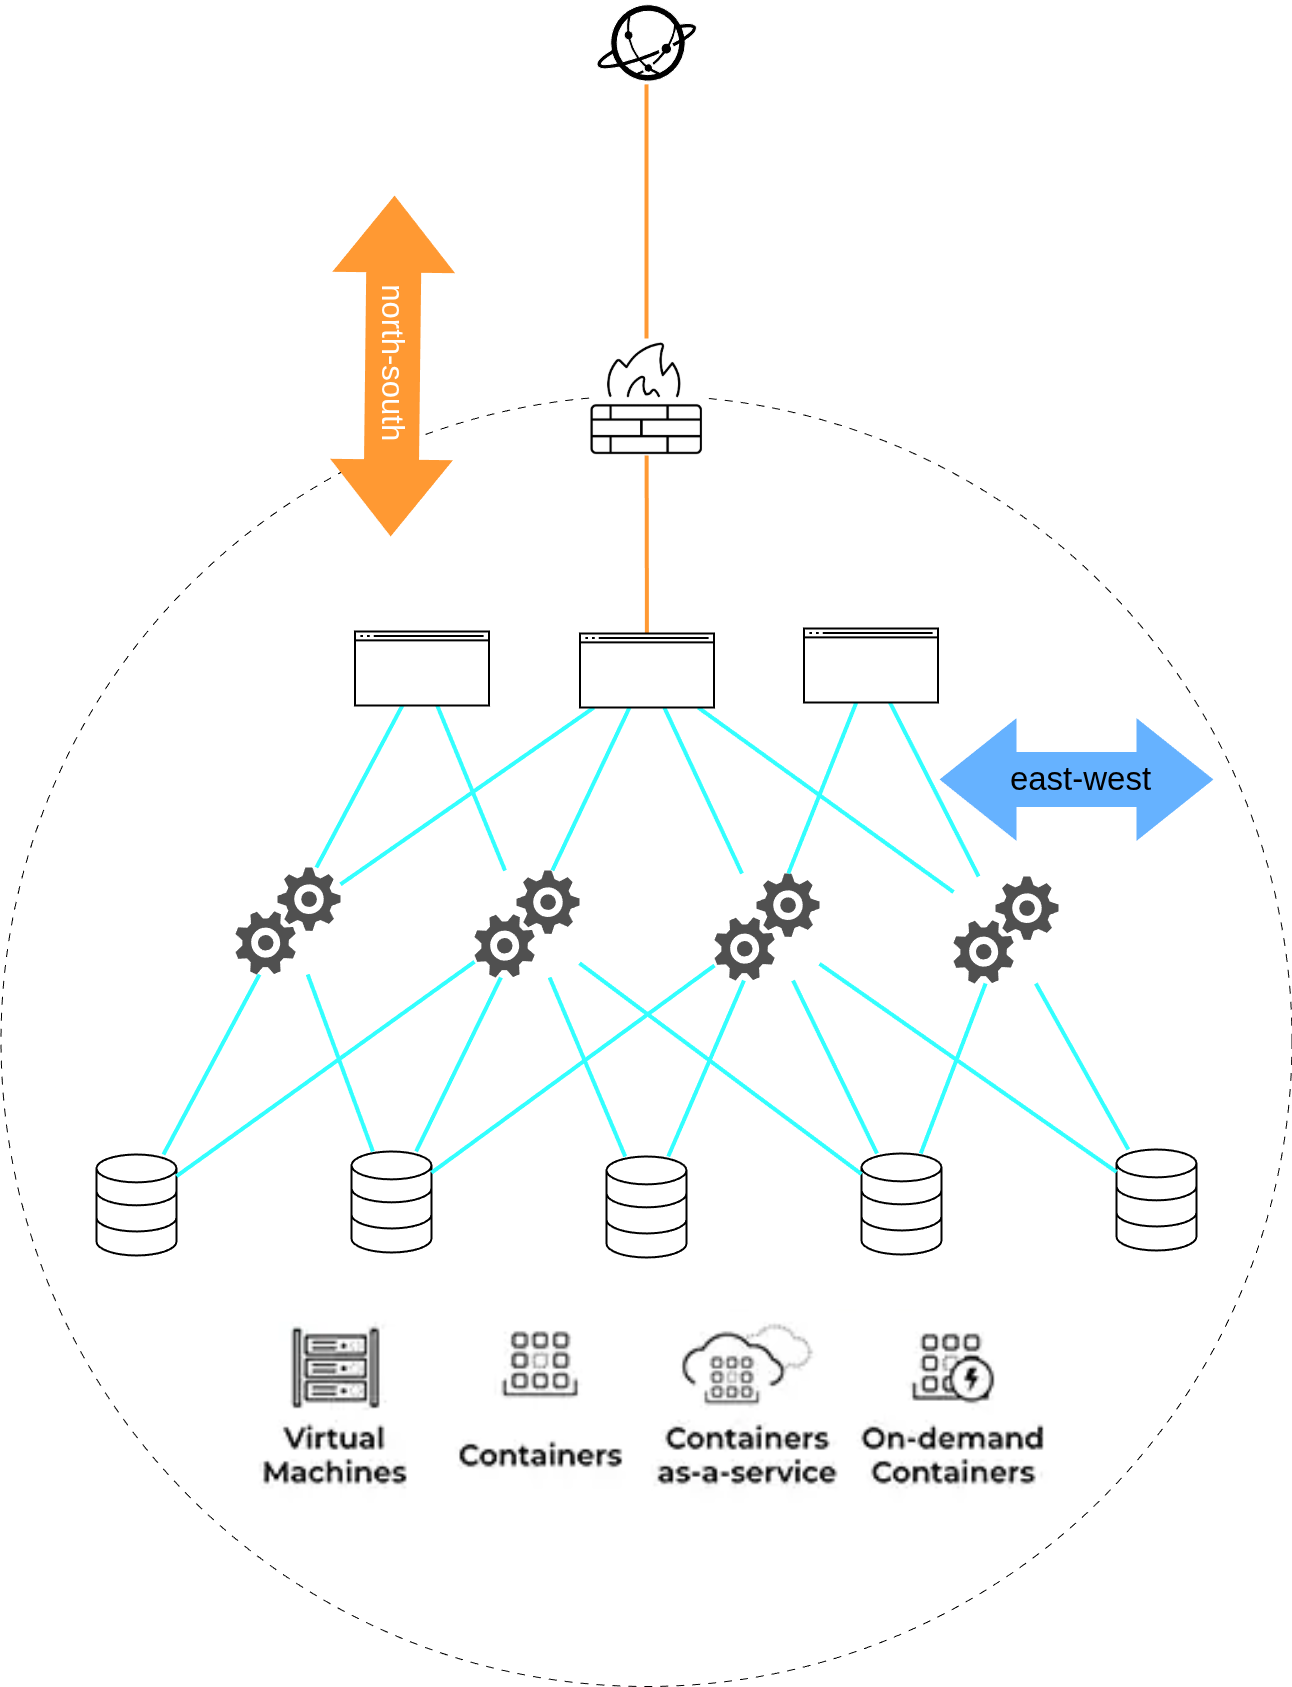
\includegraphics[width=0.7\textwidth]{images/nsew.png}
    \caption{Lưu lượng \textit{North-South} (từ Internet vào hệ thống) và \textit{East-West} (giữa các dịch vụ nội bộ)}
    \label{fig:nsew}
\end{figure}


\subsection{Zero Trust: Định nghĩa và phân biệt các cấp độ}

Đối mặt với sự thất bại của mô hình Perimeter, khái niệm Zero Trust (Không tin cậy) được John Kindervag đề xuất năm 2010 tại Forrester Research \cite{kindervag2010build}, và sau đó được chuẩn hóa thành kiến trúc tham chiếu trong \textbf{NIST SP 800-207} \cite{nist800207}.

Cần phân biệt rõ ba cấp độ của khái niệm này:

\begin{table}[H]
\centering
\caption{Phân biệt Zero Trust, ZTA và ZTE}
\label{tab:zt_levels}
\begin{tabularx}{\textwidth}{|l|l|X|}
\hline
\textbf{Thuật ngữ} & \textbf{Viết tắt} & \textbf{Định nghĩa} \\
\hline
Zero Trust & ZT & \textbf{Triết lý bảo mật:} ``Không bao giờ tin cậy, luôn luôn xác minh'' (\textit{Never trust, always verify}). Đây là tập hợp các nguyên tắc tư duy, không phải sản phẩm hay công nghệ cụ thể. \\
\hline
Zero Trust Architecture & ZTA & \textbf{Kiến trúc:} Bản thiết kế hệ thống áp dụng triết lý ZT. NIST SP 800-207 định nghĩa mô hình logic gồm PE (Policy Engine), PA (Policy Administrator) và PEP (Policy Enforcement Point). \\
\hline
Zero Trust Environment & ZTE & \textbf{Môi trường vận hành:} Hệ thống thực tế đang chạy, nơi kiến trúc ZTA đã được triển khai và đang thực thi chính sách. Đây là kết quả cuối cùng mà Chương 3 của đồ án hướng tới. \\
\hline
\end{tabularx}
\end{table}

Triết lý cốt lõi của Zero Trust dựa trên hai giả định nền tảng:
\begin{enumerate}
    \item \textbf{Mạng luôn bị coi là đã bị xâm nhập} — hệ thống không bao giờ tin rằng mạng nội bộ an toàn.
    \item \textbf{Mọi kết nối đều thù địch cho đến khi được xác minh} — bất kể nguồn gốc (nội bộ hay bên ngoài), mọi request đều phải trải qua xác thực, ủy quyền và đánh giá rủi ro.
\end{enumerate}


%==============================================================================
% 1.2  KIẾN TRÚC LOGIC CỦA ZTA THEO NIST
%==============================================================================
\section{Kiến trúc logic của ZTA theo NIST SP 800-207}

\subsection{7 nguyên lý cốt lõi (Seven Tenets)}

NIST SP 800-207 định nghĩa 7 nguyên lý nền tảng mà mọi triển khai ZTA phải tuân thủ \cite{nist800207}:

\begin{table}[H]
\centering
\caption{7 nguyên lý cốt lõi Zero Trust theo NIST SP 800-207}
\label{tab:seven_tenets}
\begin{tabularx}{\textwidth}{|c|p{4cm}|X|}
\hline
\textbf{\#} & \textbf{Nguyên lý} & \textbf{Nội dung} \\
\hline
1 & Mọi thứ đều là tài nguyên & Máy chủ, container, API endpoint, database — tất cả đều là tài nguyên cần bảo vệ riêng biệt. \\
\hline
2 & Bảo mật không phụ thuộc vị trí mạng & Giao tiếp nội bộ (cùng subnet) vẫn phải mã hóa và xác thực như traffic từ Internet. \\
\hline
3 & Cấp quyền theo phiên (\textit{per-session}) & Quyền truy cập được cấp tối thiểu (Least Privilege), đánh giá lại mỗi phiên, thu hồi ngay sau khi hoàn thành. \\
\hline
4 & Chính sách truy cập động & Quyết định dựa trên danh tính + trạng thái thiết bị + hành vi + thời gian + vị trí — không phải IP tĩnh. \\
\hline
5 & Giám sát toàn bộ tài sản & Liên tục đánh giá tính toàn vẹn và trạng thái tuân thủ của mọi thiết bị/workload. \\
\hline
6 & Xác thực liên tục & Không chỉ xác thực lần đầu — xác thực lại khi thực hiện hành động nhạy cảm hoặc khi ngữ cảnh thay đổi. \\
\hline
7 & Thu thập tối đa dữ liệu & Logs, metrics, traces từ mọi thành phần — làm đầu vào cho PE ra quyết định và cải thiện chính sách. \\
\hline
\end{tabularx}
\end{table}


\subsection{Mô hình logic bắt buộc: PE, PA và PEP}

NIST SP 800-207 định nghĩa một \textbf{kiến trúc logic} dựa trên nguyên tắc tách biệt hoàn toàn giữa \textbf{Mặt phẳng điều khiển (Control Plane)} — nơi ra quyết định, và \textbf{Mặt phẳng dữ liệu (Data Plane)} — nơi luồng dữ liệu thực tế di chuyển. Tiêu chuẩn này không ép buộc doanh nghiệp phải sử dụng một loại phần cứng hay phần mềm cụ thể nào \cite{nist800207}.

Ba thành phần logic bắt buộc:

\begin{itemize}
    \item \textbf{Policy Engine (PE) — Động cơ Chính sách:} ``Bộ não'' của hệ thống ZTA. PE tiếp nhận request, tổng hợp dữ liệu từ nhiều nguồn (danh tính, trạng thái thiết bị, threat intelligence, lịch sử hành vi) và ra quyết định \texttt{Allow} hoặc \texttt{Deny}. PE không trực tiếp chặn hay cho phép gói tin — nó chỉ \textit{ra quyết định}.

    \item \textbf{Policy Administrator (PA) — Quản trị Chính sách:} ``Cánh tay nối dài'' thực thi quyết định của PE. Khi PE quyết định Allow, PA tạo phiên kết nối (session token, credential tạm thời) hoặc cấu hình PEP để mở đường. Khi PE quyết định Deny, PA thu hồi session, revoke credential, hủy kết nối.

    \item \textbf{Policy Enforcement Point (PEP) — Điểm Thực thi Chính sách:} Thành phần nằm trực tiếp trên đường dữ liệu, tiếp xúc với mọi gói tin. PEP chặn request, hỏi PE/PA, và thực thi quyết định (forward hoặc drop). PEP có thể là API Gateway, eBPF agent, hoặc proxy sidecar.
\end{itemize}

\begin{figure}[H]
    \centering
    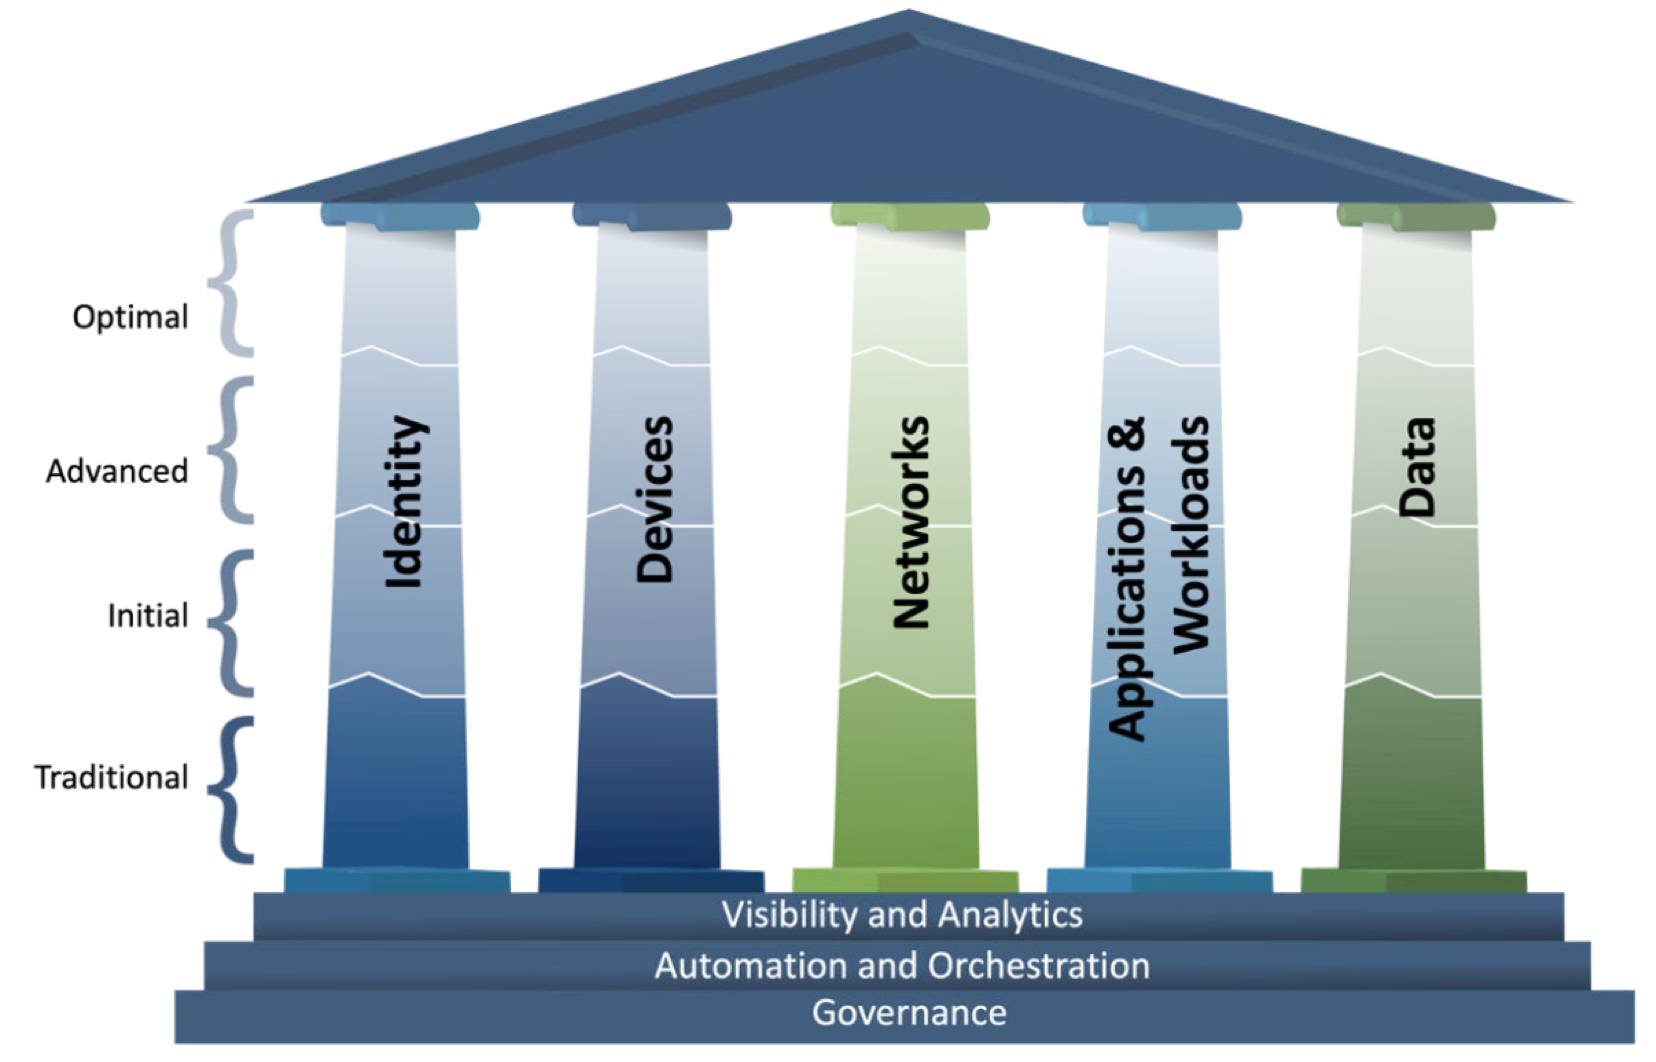
\includegraphics[width=0.9\textwidth]{images/ZTAPillars.png}
    \caption{5 trụ cột của ZTA theo NIST SP 800-207}
    \label{fig:ZTAPillars}
\end{figure}


\subsection{Vòng đời quyết định truy cập}

Mỗi request trong hệ thống ZTA đều trải qua vòng đời 5 bước:

\begin{enumerate}
    \item \textbf{Chủ thể gửi request:} Người dùng hoặc workload gửi request truy cập tài nguyên.
    \item \textbf{PEP chặn request:} PEP nằm trên đường dữ liệu, ngưng luồng và chuyển thông tin đến PE.
    \item \textbf{PE đánh giá đa chiều:} PE tổng hợp: danh tính (JWT claims, SPIFFE ID) + trạng thái thiết bị (MDM) + threat intelligence (IoC feeds) + hành vi lịch sử (UEBA) → ra quyết định Allow/Deny.
    \item \textbf{PA thực thi:} Nếu Allow → PA tạo session/credential tạm thời, cấu hình PEP mở đường. Nếu Deny → PA từ chối, ghi log.
    \item \textbf{Giám sát liên tục:} Sau khi cho phép, hệ thống vẫn giám sát phiên. Nếu phát hiện anomaly → PE ra quyết định Deny mới → PA thu hồi quyền giữa chừng (\textit{continuous re-evaluation}).
\end{enumerate}


\subsection{Ba hướng triển khai theo NIST}

Tùy mục tiêu bảo vệ — con người, máy chủ hay ứng dụng — NIST chia ra 3 hướng tiếp cận \cite{nist800207}:

\begin{itemize}
    \item \textbf{Enhanced Identity Governance (Quản trị Danh tính Nâng cao):} Lấy \textit{danh tính} làm trung tâm. Mọi quyết định truy cập dựa trên ``chủ thể là ai'' + ``thuộc tính gì'' (role, department, clearance level). Phù hợp với tổ chức có IdP mạnh (Okta, Azure AD, Keycloak).

    \item \textbf{Micro-segmentation (Phân đoạn Vi mô):} Lấy \textit{mạng} làm trung tâm. Chia mạng thành các phân đoạn cực nhỏ bao quanh từng tài nguyên hoặc nhóm tài nguyên. Ngăn chặn di chuyển ngang bằng cách đảm bảo kẻ tấn công chiếm 1 phân đoạn vẫn không thể vươn sang phân đoạn kế bên.

    \item \textbf{Software Defined Perimeter (Chu vi Định nghĩa bằng Phần mềm — SDP):} Lấy \textit{ứng dụng} làm trung tâm. Tài nguyên hoàn toàn ``tàng hình'' cho đến khi chủ thể xác thực thành công — network controller động thiết lập đường truyền an toàn giữa client và tài nguyên.
\end{itemize}

\textbf{Trong thực tế}, các tổ chức thường kết hợp cả 3 hướng: Identity Governance cho luồng North-South (người dùng → hệ thống), Micro-segmentation cho luồng East-West (service → service), và SDP cho truy cập từ xa.


%==============================================================================
% 1.3  ZTA LÀ HỆ SINH THÁI
%==============================================================================
\section{ZTA là hệ sinh thái, không phải sản phẩm}

\subsection{Tại sao không có ``một sản phẩm ZTA duy nhất''?}

Một trong những quan niệm sai lầm phổ biến nhất là coi Zero Trust như một sản phẩm phần mềm ``đóng gói'' có thể mua và cài đặt một lần. Thực tế, ZTA là một \textbf{triết lý thiết kế và lộ trình kiến trúc}, không phải một sản phẩm đơn lẻ \cite{nist800207}. Không có nhà cung cấp nào (kể cả Cisco, Palo Alto hay Microsoft) có thể cung cấp 100\% các thành phần logic NIST trong một công cụ duy nhất mà không bộc lộ hai rủi ro:

\begin{itemize}
    \item \textbf{Vendor Lock-in (Bị kẹt nhà cung cấp):} Toàn bộ hệ thống phụ thuộc vào một nhà cung cấp. Nếu nhà cung cấp tăng giá, ngừng hỗ trợ, hoặc bị xâm nhập (như SolarWinds) — toàn bộ chiến lược ZTA sụp đổ.
    \item \textbf{Single Point of Failure:} Một lỗ hổng trong sản phẩm duy nhất đó ảnh hưởng toàn bộ các lớp bảo vệ, từ định danh đến thực thi đến giám sát.
\end{itemize}

\subsection{Tiếp cận ``Best-of-Breed'' với công nghệ mã nguồn mở}

Đồ án lựa chọn tiếp cận \textbf{Best-of-Breed} — chọn công cụ tốt nhất cho từng thành phần logic NIST, ưu tiên hệ sinh thái mã nguồn mở thuộc Cloud Native Computing Foundation (CNCF):

\begin{table}[H]
\centering
\caption{Ánh xạ thành phần logic NIST sang công nghệ mã nguồn mở}
\label{tab:nist_cncf_mapping}
\begin{tabularx}{\textwidth}{|p{2.8cm}|p{2.8cm}|X|}
\hline
\textbf{Thành phần NIST} & \textbf{Công nghệ} & \textbf{Vai trò} \\
\hline
PE (Policy Engine) & OPA/Rego + Keycloak & Ra quyết định truy cập dựa trên thuộc tính đa chiều (ABAC). \\
\hline
PA (Policy Admin) & HashiCorp Vault & Cấp phát credential động (JIT), thu hồi khi hết TTL, quản lý secrets. \\
\hline
PEP — North-South & Kong Gateway & API Gateway xác thực JWT Keycloak trên từng route, proxy đến backend. \\
\hline
PEP — East-West (L3-L7) & Cilium eBPF & Thực thi network policy tại kernel: L3/L4 (IP, port) + L7 (HTTP method, path). \\
\hline
PEP — Runtime & Tetragon eBPF & Giám sát syscall bên trong container, SIGKILL tiến trình đáng ngờ. \\
\hline
Identity — User & Keycloak & IdP cấp JWT (OIDC) cho người dùng qua OAuth 2.0 flow. \\
\hline
Identity — Workload & K8s ServiceAccount + SPIFFE & Định danh gắn chặt vào workload, cryptographic binding. \\
\hline
Observability & EFK + Prometheus + Grafana & Centralized logging, metrics thu thập, dashboard giám sát. \\
\hline
\end{tabularx}
\end{table}

\textbf{Ưu điểm:}
\begin{itemize}
    \item Mỗi thành phần có thể thay thế độc lập — ví dụ: đổi từ Keycloak sang Okta mà không ảnh hưởng Cilium hay Vault.
    \item Không bị vendor lock-in — toàn bộ stack là mã nguồn mở.
    \item Phù hợp với môi trường Cloud Native / Kubernetes — các công nghệ đều là CNCF graduated/incubating.
\end{itemize}


%==============================================================================
% 1.4  MÔ HÌNH ĐE DỌA
%==============================================================================
\section{Mô hình đe dọa trước khi triển khai ZTA}

\subsection{Bề mặt tấn công của Microservices}

Kiến trúc Microservices thay đổi hoàn toàn bề mặt tấn công so với Monolith:

\begin{itemize}
    \item \textbf{Khủng hoảng định danh:} Định danh đã trở thành vành đai mới và là mục tiêu hàng đầu. Thông tin xác thực bị thỏa hiệp chiếm khoảng 20,5\% các vụ vi phạm dữ liệu \cite{gilman2017zero}.
    \item \textbf{Secrets sprawl:} Mật khẩu database, API keys, TLS certificates nằm rải rác trong file \texttt{.env}, ConfigMaps, environment variables — mỗi điểm là một vector tấn công tiềm năng.
    \item \textbf{Luồng East-West không kiểm soát:} Khi service gọi service qua HTTP plaintext nội bộ, kẻ tấn công thực hiện ARP Spoofing hoặc Man-in-the-Middle có thể đọc toàn bộ payload.
    \item \textbf{Shared infrastructure:} Nhiều service chạy trên cùng node vật lý, chia sẻ kernel — container escape = kiểm soát toàn bộ node.
\end{itemize}


\subsection{Bảng đe dọa và biện pháp đối phó tương ứng}

\begin{table}[H]
\centering
\caption{Mô hình đe dọa và biện pháp ZTA tương ứng}
\label{tab:threat_countermeasure}
\begin{tabularx}{\textwidth}{|p{3cm}|X|X|}
\hline
\textbf{Đe dọa} & \textbf{Mô tả} & \textbf{Biện pháp ZTA} \\
\hline
Credential Theft & Đánh cắp mật khẩu database hoặc API key từ file \texttt{.env} & Vault JIT: credential tạm thời TTL 1h, auto-revoke \\
\hline
Lateral Movement & Di chuyển ngang từ Pod bị xâm nhập sang service khác & Cilium Default Deny + micro-segmentation theo ServiceAccount \\
\hline
API Abuse & Gọi API nội bộ không xác thực để truy cập dữ liệu trái phép & Kong JWT Gateway + Cilium L7 HTTP Policy \\
\hline
Privilege Escalation & Leo thang đặc quyền từ user thường lên admin & ABAC with least privilege + continuous re-evaluation \\
\hline
Data Exfiltration & Trích xuất dữ liệu nhạy cảm qua kênh outbound & eBPF egress policy + EFK anomaly detection \\
\hline
Supply Chain Attack & Cài mã độc vào image hoặc dependency (kiểu SolarWinds) & Container image scanning + runtime enforcement (Tetragon) \\
\hline
\end{tabularx}
\end{table}


\subsection{Ánh xạ MITRE ATT\&CK cho Kubernetes}

\begin{table}[H]
\centering
\caption{Ánh xạ kỹ thuật tấn công MITRE ATT\&CK sang lớp ZTA phòng thủ}
\label{tab:mitre_mapping}
\begin{tabularx}{\textwidth}{|p{2.5cm}|p{3cm}|X|}
\hline
\textbf{Giai đoạn MITRE} & \textbf{Kỹ thuật K8s} & \textbf{Lớp ZTA phòng thủ} \\
\hline
Initial Access & Exposed Dashboard, Compromised Image & PEP Biên (Kong JWT) + Image Scanning \\
\hline
Execution & Exec into Container, New Container & PEP Runtime (Tetragon) — block \texttt{sys\_execve} \\
\hline
Persistence & Backdoor Container, Writable hostPath & Cilium Egress Deny + Read-only rootfs \\
\hline
Privilege Escalation & Privileged Container, hostPID & K8s Pod Security Standards + OPA Gatekeeper \\
\hline
Lateral Movement & Access K8s API, Service Discovery & Cilium Default Deny + L7 micro-segmentation \\
\hline
Collection & Sensitive Data in Secrets & Vault Dynamic Secrets + tmpfs \\
\hline
Exfiltration & Transfer to Cloud Account & eBPF Egress Policy + EFK alerting \\
\hline
\end{tabularx}
\end{table}


\subsection{So sánh ZTA với mô hình Perimeter-based}

\begin{table}[H]
\centering
\caption{So sánh mô hình bảo mật truyền thống và Kiến trúc Zero Trust}
\label{tab:zta_vs_perimeter}
\begin{tabularx}{\textwidth}{|l|X|X|}
\hline
\rowcolor[HTML]{EFEFEF}
\textbf{Tiêu chí} & \textbf{Perimeter-based} & \textbf{Zero Trust Architecture} \\
\hline
Giả định tin cậy & Tin tưởng mặc định mọi thực thể bên trong mạng & Không tin tưởng bất kỳ thực thể nào \\
\hline
Cơ chế xác thực & Một lần tại cổng vào & Liên tục, đa yếu tố, theo từng phiên \\
\hline
Quyết định truy cập & Dựa trên IP, subnet & Dựa trên danh tính + ngữ cảnh + rủi ro \\
\hline
Chống Lateral Movement & Rất yếu & Micro-segmentation + per-request enforcement \\
\hline
Secrets Management & Static (file .env) & Dynamic (Vault JIT, TTL, auto-revoke) \\
\hline
Observability & Chỉ log biên & Centralized: logs + metrics + traces \\
\hline
\end{tabularx}
\end{table}


\vspace{0.5cm}

\begin{leftbar}
\textbf{Cầu nối sang Chương 2:} Chương 1 đã xác lập nền tảng lý luận về kiến trúc Zero Trust: từ sự thất bại của mô hình Perimeter, qua 7 nguyên lý NIST và kiến trúc logic PE/PA/PEP, đến ánh xạ sơ bộ sang công nghệ mã nguồn mở và mô hình đe dọa. Tuy nhiên, việc triển khai ZTA trong môi trường \textit{Microservices trên Kubernetes} đặt ra những thách thức đặc thù mà lý thuyết chung chưa thể giải đáp — đặc biệt là bài toán PEP placement, ephemeral workload identity, ``thuế Sidecar'' và ngập lụt dữ liệu quan sát. Chương 2 sẽ phân tích những thách thức này và đề xuất một khung kiến trúc ZTA 5 lớp cụ thể cho hệ thống Microservices.
\end{leftbar}
\chapter{Ứng dụng Zero Trust bảo mật hệ thống Microservices}

%==============================================================================
% 2.1 BÀI TOÁN BẢO MẬT ĐẶC THÙ
%==============================================================================
\section{Bài toán bảo mật đặc thù của hệ thống Microservices}

Kiến trúc Microservices phân rã ứng dụng thành nhiều dịch vụ độc lập, mỗi dịch vụ đảm nhiệm một chức năng nghiệp vụ riêng và giao tiếp với nhau thông qua mạng \parencite{lewis_fowler_2014}. Cách tiếp cận này giúp tăng khả năng mở rộng, triển khai độc lập và nâng cao tính linh hoạt trong quá trình phát triển phần mềm. Tuy nhiên, việc gia tăng số lượng thành phần phân tán cũng làm mở rộng đáng kể bề mặt tấn công của hệ thống so với mô hình ứng dụng nguyên khối truyền thống.

Trong thực tế, các hệ thống Microservices thường được triển khai trên nền tảng điều phối container như Kubernetes nhằm tự động hóa quá trình vận hành, mở rộng và phục hồi dịch vụ. Mặc dù mang lại nhiều lợi ích về mặt quản trị hạ tầng, môi trường này đồng thời tạo ra các thách thức bảo mật mới liên quan đến định danh thực thể, bảo vệ lưu lượng nội bộ, quản lý thông tin xác thực và giám sát hành vi tại thời điểm chạy.

Tiêu chuẩn NIST SP 800-204 chỉ ra rằng môi trường Microservices làm gia tăng đáng kể mức độ phụ thuộc vào giao tiếp mạng giữa các dịch vụ, khiến giả định về một mạng nội bộ đáng tin cậy không còn phù hợp \parencite{nist800204_microservices}. Trong bối cảnh đó, các cơ chế bảo mật tập trung tại biên mạng không còn đủ khả năng bảo vệ hệ thống trước các cuộc tấn công xuất phát từ bên trong hoặc các hành vi di chuyển ngang giữa các thành phần đã bị xâm phạm.

Do đó, trước khi xây dựng kiến trúc Zero Trust cho hệ thống Microservices, cần phân tích các thách thức bảo mật đặc thù phát sinh từ đặc tính phân tán, môi trường điều phối Kubernetes và chuỗi cung ứng phần mềm. Kết quả phân tích này là cơ sở để xác định các yêu cầu kỹ thuật mà kiến trúc đề xuất cần đáp ứng.


%------------------------------------------------------------------------------
\subsection{Thách thức định danh và quản lý thông tin xác thực}
%------------------------------------------------------------------------------

Trong kiến trúc Microservices, mỗi dịch vụ cần xác thực danh tính của các dịch vụ khác trước khi trao đổi dữ liệu hoặc truy cập tài nguyên. Quá trình này làm phát sinh số lượng lớn thông tin xác thực như khóa API, chứng chỉ số, mật khẩu dịch vụ hoặc mã truy cập tạm thời. Khi quy mô hệ thống tăng lên, việc quản lý các thông tin này trở nên phức tạp và dễ dẫn đến tình trạng phân tán thông tin xác thực trên nhiều thành phần khác nhau.

Một thực tiễn phổ biến nhưng tiềm ẩn nhiều rủi ro là lưu trữ trực tiếp thông tin xác thực trong mã nguồn, tệp cấu hình hoặc biến môi trường. Nếu một thành phần bị xâm phạm, tác nhân tấn công có thể thu thập các thông tin này để mở rộng phạm vi truy cập sang các dịch vụ khác trong hệ thống. Trong môi trường Microservices, một thông tin xác thực bị lộ thường không chỉ ảnh hưởng đến một dịch vụ đơn lẻ mà còn có thể tác động đến toàn bộ chuỗi phụ thuộc giữa các dịch vụ.

Bên cạnh đó, các hệ thống quản lý bí mật tập trung cũng phải đối mặt với bài toán Secret Zero \parencite{vault_docs}. Đây là vấn đề xác thực ban đầu đối với chính hệ thống quản lý bí mật. Nếu thông tin xác thực gốc dùng để truy cập kho bí mật bị lộ hoặc bị đánh cắp, toàn bộ cơ chế bảo vệ phía sau có thể bị vô hiệu hóa.

Những thách thức này cho thấy hệ thống cần một cơ chế định danh độc lập với địa chỉ mạng, đồng thời hỗ trợ cấp phát, luân chuyển và thu hồi thông tin xác thực một cách tự động trong suốt vòng đời hoạt động của thực thể.

%------------------------------------------------------------------------------
\subsection{Thách thức từ môi trường điều phối Kubernetes}
%------------------------------------------------------------------------------

Kubernetes cung cấp khả năng tự động triển khai, mở rộng và phục hồi ứng dụng, tuy nhiên các đặc tính này đồng thời tạo ra nhiều yêu cầu bảo mật mới so với môi trường triển khai truyền thống.

Trước hết, các Pod được tạo mới, thay thế hoặc thu hồi liên tục trong quá trình vận hành. Tính chất ngắn hạn này khiến địa chỉ IP và vị trí thực thi của các khối lượng công việc thay đổi thường xuyên \parencite{k8s_pod_lifecycle}. Do đó, việc sử dụng địa chỉ mạng như một thuộc tính nhận dạng trở nên kém hiệu quả, đặc biệt trong các cơ chế kiểm soát truy cập hoặc thực thi chính sách bảo mật.

Bên cạnh đó, Kubernetes sử dụng cơ chế phân quyền dựa trên RBAC để kiểm soát quyền truy cập vào tài nguyên của cụm. Việc cấu hình quyền hạn không phù hợp cho người dùng, ServiceAccount hoặc thành phần tự động hóa có thể tạo điều kiện cho tác nhân tấn công mở rộng phạm vi kiểm soát sau khi xâm nhập thành công \parencite{kubernetes_docs}. Các quyền có mức ảnh hưởng cao như tạo Pod đặc quyền, gắn ServiceAccount hoặc thao tác với tài nguyên điều phối có thể trở thành con đường leo thang đặc quyền trong cụm.

Những đặc điểm trên đặt ra yêu cầu phải tách biệt khái niệm định danh khỏi thông tin hạ tầng động, đồng thời áp dụng cơ chế ủy quyền tập trung và nhất quán trên toàn bộ môi trường điều phối.

%------------------------------------------------------------------------------
\subsection{Thách thức bảo mật mạng nội bộ}
%------------------------------------------------------------------------------

Khác với kiến trúc nguyên khối, phần lớn các tương tác trong hệ thống Microservices được thực hiện thông qua mạng nội bộ giữa các dịch vụ. Điều này làm gia tăng đáng kể lưu lượng East-West và biến mạng nội bộ thành một trong những bề mặt tấn công quan trọng nhất của hệ thống.

Trong trường hợp một dịch vụ bị thỏa hiệp, tác nhân tấn công có thể lợi dụng các kết nối hợp lệ đã tồn tại để thực hiện trinh sát, thu thập thông tin hoặc di chuyển ngang sang các thành phần khác. Mức độ rủi ro càng gia tăng khi các dịch vụ mặc định tin cậy lẫn nhau chỉ vì cùng nằm trong một cụm Kubernetes hoặc cùng thuộc một vùng mạng.

Một giải pháp thường được áp dụng là mã hóa toàn bộ lưu lượng nội bộ bằng cơ chế xác thực hai chiều. Tuy nhiên, việc bổ sung các lớp kiểm soát bảo mật trên đường truyền cũng có thể làm gia tăng chi phí xử lý và độ trễ truyền thông. Do đó, hệ thống cần đạt được sự cân bằng giữa yêu cầu bảo mật, khả năng mở rộng và hiệu năng vận hành.

Những thách thức này cho thấy việc bảo vệ mạng nội bộ không chỉ dừng ở mã hóa lưu lượng mà còn đòi hỏi khả năng xác thực danh tính, thực thi chính sách truy cập và kiểm soát giao tiếp giữa các thực thể ở mức chi tiết.

%------------------------------------------------------------------------------
\subsection{Thách thức giám sát và bảo vệ tại thời điểm chạy}
%------------------------------------------------------------------------------

Các biện pháp bảo mật truyền thống như kiểm tra mã nguồn, quét lỗ hổng hoặc đánh giá cấu hình chủ yếu được thực hiện trước khi hệ thống đi vào vận hành. Mặc dù giúp giảm thiểu nhiều nguy cơ bảo mật, các biện pháp này không đủ khả năng phát hiện những hành vi phát sinh trong quá trình thực thi.

Trong thực tế, tác nhân tấn công có thể khai thác các lỗ hổng chưa được công bố, thực thi mã độc trực tiếp trong bộ nhớ hoặc sử dụng các lời gọi hệ thống bất thường để vượt qua các cơ chế bảo vệ hiện có. Các hoạt động này thường không để lại dấu hiệu rõ ràng trên mã nguồn hoặc container image đã được kiểm tra trước đó.

Bên cạnh đó, các container trên cùng một nút tính toán chia sẻ chung nhân hệ điều hành. Những lỗ hổng tại lớp runtime hoặc nhân hệ điều hành có thể bị khai thác để thực hiện các kỹ thuật vượt thoát container và chiếm quyền kiểm soát máy chủ lưu trữ \parencite{cve_2024_21626,cve_2022_0847}.

Do đó, hệ thống cần khả năng quan sát liên tục đối với các hoạt động diễn ra tại thời điểm chạy, bao gồm hành vi tiến trình, tương tác mạng và các lời gọi hệ thống quan trọng. Dữ liệu quan sát được phải có khả năng hỗ trợ phát hiện bất thường và cung cấp ngữ cảnh cho quá trình ra quyết định bảo mật.

%------------------------------------------------------------------------------
\subsection{Thách thức từ chuỗi cung ứng phần mềm}
%------------------------------------------------------------------------------

Mỗi khối lượng công việc triển khai trong Kubernetes thường được xây dựng từ nhiều thành phần phần mềm khác nhau như hệ điều hành nền, thư viện phụ thuộc, container image và các gói mã nguồn từ bên thứ ba. Điều này khiến chuỗi cung ứng phần mềm trở thành một mục tiêu hấp dẫn đối với tác nhân tấn công.

Một container image chứa mã độc, thư viện bị cài cắm hoặc được phát hành từ nguồn không đáng tin cậy có thể đưa mã thực thi độc hại trực tiếp vào môi trường sản xuất mà không cần khai thác bất kỳ lỗ hổng nào trên hệ thống đang vận hành. Các cuộc tấn công vào chuỗi cung ứng phần mềm trong những năm gần đây cho thấy việc bảo vệ môi trường thực thi là chưa đủ nếu nguồn gốc của khối lượng công việc không được xác minh.

Do đó, ngoài việc kiểm tra lỗ hổng bảo mật, hệ thống cần có khả năng xác thực nguồn gốc, tính toàn vẹn và trạng thái phê duyệt của các thành phần trước khi cho phép triển khai vào môi trường vận hành.

%------------------------------------------------------------------------------
\subsection{Phân tích bề mặt tấn công theo mô hình MITRE ATT\&CK}
%------------------------------------------------------------------------------

Các thách thức bảo mật đã phân tích ở các mục trước phản ánh những đặc điểm nội tại của kiến trúc Microservices và môi trường Kubernetes. Tuy nhiên, để đánh giá mức độ liên hệ giữa các thách thức này với các mối đe dọa trong thực tế, cần đối chiếu chúng với một mô hình phân tích tấn công có tính hệ thống và được thừa nhận rộng rãi.

Trong phạm vi đồ án, khung MITRE ATT\&CK dành cho Container được sử dụng làm cơ sở tham chiếu \parencite{mitre_containers}. Đây là cơ sở tri thức mô tả hành vi của tác nhân tấn công thông qua tập hợp các chiến thuật và kỹ thuật đã được quan sát trong thực tế. Đối với môi trường container và Kubernetes, MITRE ATT\&CK cung cấp một góc nhìn toàn diện về chuỗi tấn công, từ giai đoạn xâm nhập ban đầu, thiết lập chỗ đứng trong hệ thống cho đến các hoạt động hậu khai thác như leo thang đặc quyền, di chuyển ngang và gây tác động lên tài nguyên.

Việc đối chiếu với MITRE ATT\&CK không nhằm liệt kê đầy đủ mọi kỹ thuật tấn công có thể xảy ra, mà tập trung xác định những thành phần hệ thống thường xuyên trở thành mục tiêu trong môi trường Microservices. Kết quả phân tích cho phép đánh giá liệu các thách thức đã được nhận diện trước đó có phản ánh đúng thực tiễn tấn công hay không, đồng thời làm cơ sở để xác định các yêu cầu kỹ thuật đối với kiến trúc Zero Trust được đề xuất.

Hình \ref{fig:mitre_containers} minh họa các chiến thuật và kỹ thuật tấn công phổ biến đối với môi trường container theo khung MITRE ATT\&CK.

\begin{figure}[H]
    \centering
    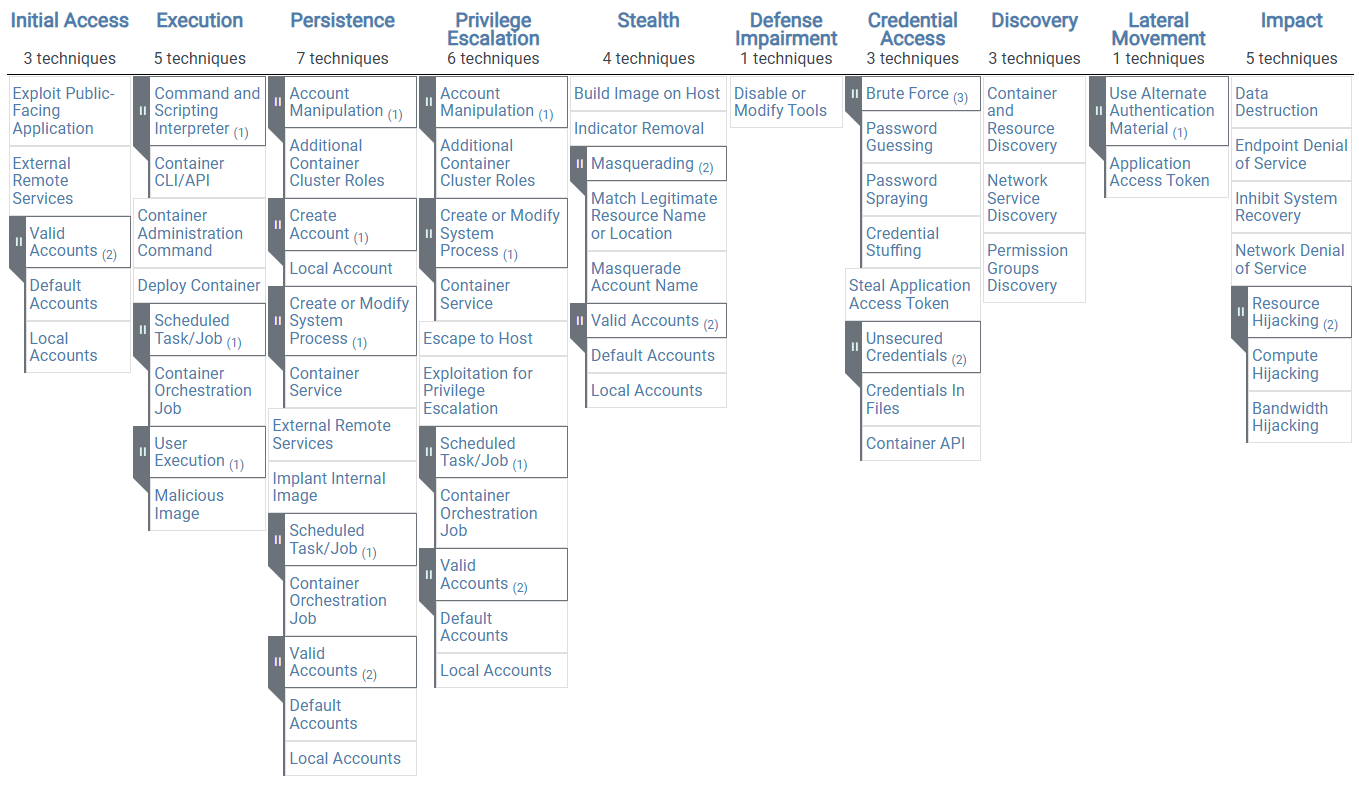
\includegraphics[width=\textwidth]{images/mitre_attack_containers.png}
    \caption[Các kỹ thuật tấn công vào môi trường Container]{Các chiến thuật và kỹ thuật tấn công đối với môi trường Container theo khung MITRE ATT\&CK \parencite{mitre_containers}.}
    \label{fig:mitre_containers}
\end{figure}

Để thuận tiện cho việc phân tích, các kỹ thuật tiêu biểu được nhóm thành hai giai đoạn chính gồm giai đoạn xâm nhập và thiết lập chỗ đứng trong hệ thống, cùng giai đoạn hậu khai thác và mở rộng phạm vi ảnh hưởng.

\begin{table}[H]
\centering
\caption{Các kỹ thuật MITRE ATT\&CK liên quan đến giai đoạn xâm nhập và thiết lập chỗ đứng}
\label{tab:mitre_phase1}
\renewcommand{\arraystretch}{1.3}
\begin{tabularx}{\textwidth}{|p{3.5cm}|X|p{4.5cm}|}
\hline
\textbf{Chiến thuật} &
\textbf{Kỹ thuật tiêu biểu} &
\textbf{Thách thức liên quan} \\
\hline

Xâm nhập ban đầu &
Khai thác ứng dụng công khai (T1190); Lạm dụng tài khoản hợp lệ (T1078) &
Định danh và quản lý thông tin xác thực \\
\hline

Thực thi &
Triển khai image chứa mã độc (T1610); Thực thi lệnh thông qua API điều phối (T1609) &
Chuỗi cung ứng phần mềm; Môi trường Kubernetes \\
\hline

Duy trì truy cập &
Tạo tác vụ định kỳ (T1053); Triển khai container chạy nền (T1525) &
Môi trường Kubernetes; Giám sát thời gian chạy \\
\hline

Ẩn mình &
Trá hình tiến trình (T1036); Xóa dấu vết hoạt động (T1070) &
Khả năng quan sát và giám sát thời gian chạy \\
\hline

Vô hiệu hóa phòng thủ &
Sửa đổi hoặc vô hiệu hóa cơ chế bảo vệ (T1562) &
Giám sát thời gian chạy; Thực thi chính sách bảo mật \\
\hline

\end{tabularx}
\end{table}

\begin{table}[H]
\centering
\caption{Các kỹ thuật MITRE ATT\&CK liên quan đến giai đoạn hậu khai thác}
\label{tab:mitre_phase2}
\renewcommand{\arraystretch}{1.3}
\begin{tabularx}{\textwidth}{|p{3.5cm}|X|p{4.5cm}|}
\hline
\textbf{Chiến thuật} &
\textbf{Kỹ thuật tiêu biểu} &
\textbf{Thách thức liên quan} \\
\hline

Leo thang đặc quyền &
Vượt thoát container hoặc khai thác đặc quyền máy chủ (T1611) &
Môi trường Kubernetes; Bảo vệ thời gian chạy \\
\hline

Truy cập thông tin nhạy cảm &
Thu thập thông tin xác thực từ tệp cấu hình hoặc biến môi trường (T1552) &
Định danh và quản lý thông tin xác thực \\
\hline

Trinh sát &
Dò quét dịch vụ và tài nguyên nội bộ (T1046, T1613) &
Bảo mật mạng nội bộ \\
\hline

Di chuyển ngang &
Lợi dụng dịch vụ nội bộ hoặc tái sử dụng thông tin xác thực (T1021) &
Bảo mật mạng nội bộ; Định danh và ủy quyền \\
\hline

Tác động &
Chiếm dụng tài nguyên điện toán (T1496); Tấn công từ chối dịch vụ (T1498) &
Khả năng chống chịu và bảo vệ tài nguyên hệ thống \\
\hline

\end{tabularx}
\end{table}


Từ kết quả phân tích, đồ án xác định bốn yêu cầu kỹ thuật cốt lõi làm cơ sở cho việc thiết kế kiến trúc Zero Trust trong các chương tiếp theo.

\begin{enumerate}[itemsep=6pt, parsep=0pt]

\item \textbf{Thiết lập định danh độc lập với hạ tầng mạng}

Trong môi trường Kubernetes, các thực thể có tính động cao, địa chỉ IP và vị trí thực thi thay đổi liên tục trong quá trình vận hành. Do đó, hệ thống cần một cơ chế định danh ổn định, có khả năng xác minh bằng mật mã học và không phụ thuộc vào thông tin định tuyến hoặc vị trí triển khai của thực thể.

\item \textbf{Quản lý vòng đời thông tin xác thực}

Thông tin xác thực cần được cấp phát, sử dụng, luân chuyển và thu hồi theo vòng đời hoạt động của thực thể. Kiến trúc phải hạn chế việc lưu trữ tĩnh các bí mật trong mã nguồn hoặc cấu hình, đồng thời bảo đảm khả năng phân phối thông tin xác thực một cách tự động và có kiểm soát.

\item \textbf{Thực thi chính sách truy cập phân tán và nhất quán}

Các quyết định truy cập không thể phụ thuộc vào một điểm kiểm soát duy nhất. Hệ thống cần khả năng thực thi chính sách tại nhiều vị trí khác nhau như lớp mạng, môi trường thực thi, thành phần ứng dụng và nền tảng điều phối, đồng thời duy trì tính nhất quán trong quá trình đánh giá và cấp quyền.

\item \textbf{Ra quyết định dựa trên ngữ cảnh và khả năng quan sát}

Việc cấp quyền truy cập cần dựa trên nhiều yếu tố hơn là danh tính của thực thể. Kiến trúc phải có khả năng thu thập dữ liệu quan sát từ môi trường vận hành, liên kết dữ liệu này với định danh tương ứng và sử dụng chúng làm đầu vào cho quá trình đánh giá rủi ro và thực thi chính sách.

\end{enumerate}

Bốn yêu cầu kỹ thuật trên phản ánh trực tiếp các thách thức bảo mật đã được nhận diện trong môi trường Microservices. Đây cũng là cơ sở để xây dựng kiến trúc logic Zero Trust được trình bày trong các mục tiếp theo của chương.


%==============================================================================
% 2.2 KIẾN TRÚC ZERO TRUST ĐỀ XUẤT
%==============================================================================
\section{Kiến trúc Zero Trust đề xuất}

Kiến trúc đề xuất hiện thực hóa ba vai trò logic của NIST SP 800-207 ---
Điểm cung cấp thông tin (PIP), Điểm quyết định chính sách (PDP) và Điểm
thực thi chính sách (PEP) --- thành năm thành phần chức năng, phân tách
theo tần suất cập nhật và vị trí trong luồng xử lý yêu cầu truy cập
\parencite{nist800207}. Thành phần 1 và Thành phần 2 đóng vai trò PIP với
hai loại ngữ cảnh khác nhau về tần suất cập nhật; Thành phần 3 là PDP;
Thành phần 4 là PEP; Thành phần 5 là PIP telemetry đóng vòng phản hồi về
Thành phần 3.

Luồng xử lý một yêu cầu truy cập diễn ra tuần tự: xác thực định danh
của thực thể, đánh giá trạng thái bảo mật hiện tại, ra quyết định cấp
quyền, thực thi quyết định tại các điểm kiểm soát, và ghi nhận sự kiện
để cập nhật ngữ cảnh cho vòng đánh giá tiếp theo.

\begin{figure}[H]
\centering
\begin{tikzpicture}[
  font=\footnotesize\sffamily,
  blk/.style={draw, rounded corners=3pt, minimum height=13mm,
               text width=12.5cm, align=left, inner sep=6pt, line width=0.6pt},
  s1/.style={blk, fill=blue!7,    draw=blue!50},
  s2/.style={blk, fill=cyan!7,    draw=cyan!50},
  s3/.style={blk, fill=orange!9,  draw=orange!60},
  s4/.style={blk, fill=green!8,   draw=green!50},
  s5/.style={blk, fill=violet!7,  draw=violet!50},
  lbl/.style={font=\scriptsize\sffamily\itshape, text=gray!65}
]

\node[s1] (s1) at (0,12.0) {
  \textbf{Thành phần 1 — Định danh và Xác thực}
  \hfill \lbl{PIP · cập nhật theo TTL chứng chỉ}\\[3pt]
  Cấp và xác minh định danh mật mã học cho mọi thực thể trước khi yêu cầu
  được xem xét. Người dùng xác thực qua giao thức OIDC và nhận mã truy cập
  ngắn hạn. Mỗi workload được cấp chứng chỉ định danh X.509 theo chuẩn
  SPIFFE, có thời gian sống ngắn và tự động gia hạn, thay thế địa chỉ IP
  làm căn cứ nhận dạng.};

\node[s2] (s2) at (0, 8.8) {
  \textbf{Thành phần 2 — Đánh giá tư thế bảo mật}
  \hfill \lbl{PIP · cập nhật theo batch và sự kiện}\\[3pt]
  Thu thập và duy trì ngữ cảnh bảo mật động của từng workload để cung cấp
  cho Thành phần 3. Bao gồm quét lỗ hổng phần mềm định kỳ trên image đang
  chạy, kiểm tra tuân thủ cấu hình và đồng bộ danh sách địa chỉ độc hại
  từ nguồn tình báo bên ngoài. Thành phần này không trực tiếp thực thi
  chính sách --- toàn bộ dữ liệu được chuyển sang Thành phần 3 để ra
  quyết định.};

\node[s3] (s3) at (0, 5.5) {
  \textbf{Thành phần 3 — Ra quyết định và Phân phối chính sách}
  \hfill \lbl{PDP · PE + PA}\\[3pt]
  Nhận định danh từ Thành phần 1 và ngữ cảnh từ Thành phần 2, áp dụng
  thuật toán đánh giá rủi ro đa chiều để xác định mức độ tin cậy và hành
  động phản hồi phù hợp. Đồng thời điều phối cấp phát thông tin xác thực
  tạm thời theo cơ chế JIT cho workload được phê duyệt --- việc tiêm thông
  tin xác thực vào môi trường thực thi được thực hiện bởi Thành phần 4.};

\node[s4] (s4) at (0, 2.3) {
  \textbf{Thành phần 4 — Thực thi chính sách}
  \hfill \lbl{PEP · biên · mạng · admission · runtime}\\[3pt]
  Thực thi quyết định từ Thành phần 3 tại bốn vị trí độc lập nhau. Tại
  biên hệ thống: kiểm tra hiệu lực mã truy cập. Tại mạng nội bộ: áp dụng
  chính sách từ chối mặc định, chỉ cho phép luồng được khai báo tường
  minh kết hợp xác thực định danh mTLS. Tại cổng nạp: kiểm tra tính toàn
  vẹn và nguồn gốc image. Tại runtime: giám sát và kiểm soát lời gọi hệ
  thống bất thường ở tầng nhân.};

\node[s5] (s5) at (0,-0.6) {
  \textbf{Thành phần 5 — Quan sát và Phản hồi thích ứng}
  \hfill \lbl{PIP · telemetry thời gian thực → Thành phần 3}\\[3pt]
  Thu thập toàn bộ sự kiện từ bốn thành phần trên và đưa trở lại Thành
  phần 3 làm ngữ cảnh cho vòng đánh giá tiếp theo. Mỗi bản ghi sự kiện
  mạng được gắn định danh thực thể thay vì địa chỉ IP. Khi phát hiện tín
  hiệu bất thường, Thành phần 3 cập nhật đánh giá rủi ro và phân phối
  chính sách mới xuống Thành phần 4 mà không cần can thiệp thủ công.};

\foreach \from/\to in {s1/s2, s2/s3, s3/s4, s4/s5}
  \draw[->, >=Latex, gray!55, line width=0.7pt] (\from) -- (\to);

\draw[->, >=Latex, dashed, gray!50, line width=0.7pt]
  (s5.east) -- ++(1.6,0) |-
  node[pos=0.25, right, font=\scriptsize\sffamily, text=gray!60,
       align=left, xshift=2pt] {Cập nhật ngữ cảnh\\cho vòng đánh giá tiếp theo}
  (s3.east);

\end{tikzpicture}
\caption{Năm thành phần chức năng của kiến trúc Zero Trust đề xuất và ánh
         xạ vào ba vai trò logic NIST SP 800-207}
\label{fig:zta_five_components}
\end{figure}

%------------------------------------------------------------------------------
\subsection{Thành phần 1 — Định danh và Xác thực}
%------------------------------------------------------------------------------

\textbf{Vai trò:} Cung cấp định danh mật mã học cho mọi thực thể trong hệ thống, thay thế địa chỉ IP làm căn cứ kiểm soát truy cập. Đây là đầu vào bắt buộc cho Thành phần 3 --- không có định danh hợp lệ thì không có quyết định cấp quyền.

\textbf{Định danh người dùng:} Người dùng xác thực qua giao thức OIDC và nhận mã truy cập dạng JWT có thời gian sống ngắn. JWT mang theo các thuộc tính phân quyền phục vụ quá trình đánh giá ở Thành phần 3.

\textbf{Định danh workload:} Mỗi workload khi khởi tạo được cấp một chứng chỉ X.509 SVID theo chuẩn SPIFFE \parencite{spiffe_spec}. Chứng chỉ có thời gian sống rất ngắn, tự động gia hạn và không phụ thuộc vào địa chỉ IP hay cấu hình mạng. Workload sử dụng SVID để xác thực lẫn nhau qua mTLS trên mạng nội bộ.

\textbf{Chế độ lỗi:} Nếu dịch vụ cấp chứng chỉ không phản hồi, các SVID hiện có vẫn hợp lệ đến hết TTL. Workload mới không thể khởi động khi chưa có SVID hợp lệ --- đây là hành vi từ chối an toàn có chủ đích.

%------------------------------------------------------------------------------
\subsection{Thành phần 2 — Đánh giá tư thế bảo mật}
%------------------------------------------------------------------------------

\textbf{Vai trò:} Thu thập và duy trì ngữ cảnh bảo mật động của từng workload để Thành phần 3 có đủ thông tin ra quyết định. Thành phần 2 không thực thi chính sách --- ranh giới này đảm bảo tính tách biệt giữa thu thập dữ liệu và ra quyết định.

\textbf{Đánh giá lỗ hổng:} Quét định kỳ các image đang chạy và sinh báo cáo lỗ hổng dưới dạng tài nguyên Kubernetes. Khi CVE mới được công bố, báo cáo cập nhật tự động mà không cần triển khai lại workload.

\textbf{Kiểm tra tuân thủ cấu hình:} Đánh giá tài nguyên Kubernetes theo tập hợp ràng buộc định nghĩa trước --- nhãn bắt buộc, cấu hình bảo mật Pod, quyền hạn tối thiểu. Kết quả được chuyển sang Thành phần 3 làm một trong các yếu tố tính điểm rủi ro.

\textbf{Tình báo đe dọa:} Đồng bộ định kỳ danh sách địa chỉ IP và tên miền độc hại từ nguồn bên ngoài. Dữ liệu này được Thành phần 3 sử dụng để phát hiện lưu lượng đến các đích đã biết là độc hại.

\textbf{Chế độ lỗi:} Nếu quá trình quét gián đoạn, kết quả cũ được giữ nguyên với trạng thái lỗi thời. Thành phần 3 tính điểm dựa trên dữ liệu này với mức tin cậy thấp hơn thay vì tự động chặn.

%------------------------------------------------------------------------------
\subsection{Thành phần 3 — Ra quyết định và Phân phối chính sách}
%------------------------------------------------------------------------------

\textbf{Vai trò:} Nhận định danh từ Thành phần 1 và ngữ cảnh từ Thành phần 2 và Thành phần 5, tính toán mức độ rủi ro, ra quyết định và phân phối quyết định đó xuống Thành phần 4. Đây là thành phần duy nhất có thể thay đổi trạng thái kiểm soát truy cập của một workload.

\textbf{Đánh giá rủi ro đa chiều:} Thay vì gán điểm phạt tuyến tính theo mức độ nghiêm trọng của lỗ hổng, Động cơ chính sách đánh giá rủi ro theo ba chiều độc lập: mức độ nghiêm trọng của lỗ hổng, khả năng khai thác qua mạng và phân cấp dịch vụ. Cơ chế đánh giá và ma trận phản hồi được trình bày chi tiết tại Mục~\ref{sec:risk_model}.

\textbf{Phân phối chính sách:} Bộ điều phối chính sách cập nhật nhãn phân cấp rủi ro trên workload và đồng bộ chính sách mạng tương ứng xuống Thành phần 4. Các điểm thực thi đối chiếu nhãn này khi xử lý lưu lượng, không cần kết nối trực tiếp về Thành phần 3 cho mỗi yêu cầu.

\textbf{Cấp phát thông tin xác thực động:} Thành phần 3 phê duyệt yêu cầu cấp thông tin xác thực tạm thời theo cơ chế JIT. Khi một workload được phê duyệt, hệ thống cấp tài khoản ngẫu nhiên với TTL ngắn. Việc tiêm thông tin xác thực vào môi trường thực thi của Pod được thực hiện bởi cơ chế sidecar thuộc Thành phần 4.

\textbf{Chế độ lỗi:} Nếu Thành phần 3 không phản hồi, các điểm thực thi ở Thành phần 4 giữ nguyên chính sách cuối cùng nhận được --- không tự động mở thêm quyền.

%------------------------------------------------------------------------------
\subsection{Thành phần 4 — Thực thi chính sách}
%------------------------------------------------------------------------------

\textbf{Vai trò:} Thực thi quyết định từ Thành phần 3 tại bốn vị trí độc lập nhau. Không điểm thực thi nào trong Thành phần 4 tự ra quyết định --- tất cả đối chiếu với chính sách được phân phối từ Thành phần 3.

\textbf{Kiểm soát biên:} Tại cửa ngõ hệ thống, mọi yêu cầu từ bên ngoài phải mang mã truy cập hợp lệ. Chính sách kiểm tra được đánh giá theo ngữ cảnh yêu cầu trước khi cho phép đi tiếp vào cluster.

\textbf{Kiểm soát mạng nội bộ:} Áp dụng chính sách từ chối mặc định trên toàn bộ lưu lượng East-West. Luồng giao tiếp giữa các workload chỉ được phép khi có khai báo tường minh trong chính sách mạng, kết hợp với xác thực định danh mTLS. Chính sách gắn theo nhãn workload, không theo địa chỉ IP --- tự động theo workload khi được tái lập lịch sang Node khác.

\textbf{Kiểm soát cổng nạp:} Mọi tài nguyên được đánh giá trước khi được chấp nhận vào cluster. Image phải có chữ ký số từ chuỗi cung ứng tin cậy. Hỗ trợ chế độ ghi nhận trước khi chuyển sang chặn tuyệt đối, cho phép tinh chỉnh cấu hình mà không gây gián đoạn dịch vụ.

\textbf{Kiểm soát runtime:} Giám sát lời gọi hệ thống tại tầng nhân thông qua cơ chế eBPF. Hoạt động hoàn toàn độc lập với không gian người dùng của Pod --- workload không thể can thiệp vào quá trình giám sát của chính nó. Hành vi bất thường được ghi nhận hoặc ngắt tùy theo chính sách cấu hình.

\textbf{Chế độ lỗi:} Nếu một điểm thực thi mất kết nối với Thành phần 3, nó giữ nguyên chính sách cuối cùng nhận được. Các điểm thực thi còn lại vẫn hoạt động độc lập nhau.

%------------------------------------------------------------------------------
\subsection{Thành phần 5 — Quan sát và Phản hồi thích ứng}
%------------------------------------------------------------------------------

\textbf{Vai trò:} Thu thập toàn bộ sự kiện từ bốn thành phần trên, tổng hợp thành ngữ cảnh mới và đưa trở lại Thành phần 3. Không có Thành phần 5, Thành phần 3 chỉ có thể phản ứng với thông tin tĩnh tại thời điểm khi tạo --- kiến trúc mất khả năng thích ứng với thay đổi trạng thái trong quá trình vận hành.

\textbf{Thu thập sự kiện:} Nhật ký từ tất cả thành phần được tập trung về một điểm. Thành phần thu thập chạy ở tầng Node thay vì đọc qua stdout của container, ngăn workload tự can thiệp vào nhật ký của chính nó.

\textbf{Quan sát luồng mạng với ngữ cảnh định danh:} Mỗi bản ghi lưu lượng mạng mang theo tên workload, namespace và quyết định của điểm thực thi thay vì chỉ địa chỉ IP. Đây là điều kiện cần để truy vết sự cố trong môi trường IP động.

\textbf{Đóng vòng phản hồi:} Khi Thành phần 5 phát hiện tín hiệu bất thường --- lỗ hổng mới từ Thành phần 2, hành vi bất thường từ Thành phần 4 --- thông tin được chuyển về Thành phần 3. Thành phần 3 tính lại đánh giá rủi ro và cập nhật chính sách xuống Thành phần 4 mà không cần can thiệp thủ công.

\textbf{Chế độ lỗi:} Mất Thành phần 5 không ảnh hưởng đến khả năng thực thi chính sách của Thành phần 4. Tuy nhiên Thành phần 3 mất nguồn cập nhật ngữ cảnh động --- hệ thống vẫn thực thi nhưng không còn phản ứng với thay đổi trạng thái mới cho đến khi Thành phần 5 phục hồi.


%------------------------------------------------------------------------------
% LUỒNG XỬ LÝ REQUEST — cuối mục 2.2
%------------------------------------------------------------------------------

\subsection{Luồng xử lý yêu cầu truy cập}
\label{subsec:request_flow}

Năm thành phần trên không hoạt động độc lập mà phối hợp theo một luồng xử lý tuần tự mỗi khi có yêu cầu truy cập. Hình~\ref{fig:request_flow} mô tả luồng này qua sáu bước khép kín.

\begin{enumerate}[itemsep=4pt, parsep=0pt]

    \item \textbf{Xác thực định danh:} Thực thể gửi yêu cầu phải chứng minh định danh bằng mật mã học trước khi yêu cầu được xem xét --- người dùng qua JWT, workload qua chứng chỉ X.509 SVID. Thành phần~1 chịu trách nhiệm bước này.

    \item \textbf{Thu thập ngữ cảnh bảo mật:} Song song với xác thực định danh, Thành phần~2 cung cấp trạng thái bảo mật hiện tại của thực thể --- lỗ hổng đã biết, mức tuân thủ cấu hình và tình báo đe dọa từ bên ngoài.

    \item \textbf{Đánh giá rủi ro:} Thành phần~3 tổng hợp định danh từ bước 1 và ngữ cảnh từ bước 2, áp dụng thuật toán đánh giá rủi ro đa chiều để xác định mức độ tin cậy của thực thể tại thời điểm yêu cầu.

    \item \textbf{Ra quyết định và phân phối chính sách:} Dựa trên kết quả đánh giá rủi ro, Thành phần~3 ra quyết định cấp quyền, hạn chế hoặc từ chối, đồng thời phân phối chính sách tương ứng xuống các    điểm thực thi.

    \item \textbf{Thực thi:} Thành phần~4 thực thi quyết định tại bốn vị trí độc lập nhau --- biên hệ thống, mạng nội bộ, cổng nạp và runtime. Yêu cầu chỉ được thông qua khi vượt qua tất cả các điểm kiểm soát phù hợp.

    \item \textbf{Ghi nhận và cập nhật ngữ cảnh:} Thành phần~5 thu thập toàn bộ sự kiện từ các bước trên và đưa trở lại Thành phần~3. Khi trạng thái bảo mật thay đổi trong quá trình vận hành, vòng đánh giá mới được kích hoạt mà không cần yêu cầu truy cập mới làm điều kiện khởi động.

\end{enumerate}

Bước 6 là điểm phân biệt căn bản giữa kiến trúc này và mô hình kiểm soát truy cập truyền thống: quyết định không kết thúc tại thời điểm cấp phép mà tiếp tục được cập nhật theo diễn biến thực tế của môi trường vận hành. Nguyên tắc điều phối từng bước trong luồng này được trình bày ở Mục~\ref{sec:operating_principles}.


%==============================================================================
% 2.3 NGUYÊN TẮC VẬN HÀNH KIẾN TRÚC
%==============================================================================
\section{Nguyên tắc vận hành kiến trúc}
\label{sec:operating_principles}

Kiến trúc năm thành phần ở Mục~\ref{sec:zta_proposed} xác định \textit{cấu trúc} của hệ thống kiểm soát. Phần này trình bày \textit{các nguyên tắc điều phối} hoạt động bên trong cấu trúc đó --- quy tắc nào chi phối việcv ra quyết định, logic nào điều chỉnh phản hồi khi rủi ro thay đổi, và chiến lược nào dẫn dắt quá trình triển khai theo giai đoạn.

%------------------------------------------------------------------------------
\subsection{Mô hình chính sách}
\label{subsec:policy_model}
%------------------------------------------------------------------------------

\textbf{Kiểm soát truy cập theo thuộc tính:} Kiến trúc áp dụng mô hình kiểm soát truy cập dựa trên thuộc tính (ABAC) \parencite{nist_abac} thay cho phân quyền tĩnh theo vai trò. Quyết định cấp quyền là hàm đánh giá của bốn biến:

\[
\text{Decision} = f(\text{Subject},\ \text{Resource},\ \text{Action},\
\text{Environment})
\]

Trong đó \texttt{Subject} mang định danh mật mã học từ Thành phần~1, \texttt{Environment} chứa trạng thái rủi ro hiện tại từ Thành phần~3, và \texttt{Action} được đánh giá theo ngữ cảnh yêu cầu cụ thể, không phải theo quyền hạn tĩnh được cấp từ trước.

\textbf{Từ chối mặc định:} Mọi luồng giao tiếp bị từ chối cho đến khi có khai báo cho phép tường minh. Nguyên tắc này áp dụng đồng đều cho lưu lượng North-South từ bên ngoài vào và lưu lượng East-West giữa các workload trong cluster. Việc chỉ mở những gì cần thiết thay vì chặn những gì nguy hiểm là sự đảo ngược căn bản so với mô hình bảo mật vành đai truyền thống.

\textbf{Chính sách dưới dạng mã nguồn:} Toàn bộ quy tắc kiểm soát được biểu diễn dưới dạng tệp cấu hình có thể kiểm soát phiên bản, kiểm thử tự động và kiểm toán. Điều này đảm bảo mọi thay đổi chính sách đều có lịch sử rõ ràng và có thể khôi phục khi cần.

%------------------------------------------------------------------------------
\subsection{Mô hình đánh giá rủi ro}
\label{sec:risk_model}
%------------------------------------------------------------------------------

\subsubsection{Hạn chế của phương pháp đánh giá tĩnh}

Cách tiếp cận phổ biến nhất trong các hệ thống bảo mật tự động là gán điểm phạt tuyến tính dựa trên mức độ nghiêm trọng của lỗ hổng:

\[
\text{score} = \max\!\Big(0,\ 100
  - 30 \cdot \frac{\text{missing\_labels}}{6}
  - 50 \cdot \mathbb{1}[\text{has\_critical\_cve}]
  - 20 \cdot \mathbb{1}[\text{has\_high\_cve}]
\Big)
\]

Cách này có ưu điểm là đơn giản và dễ triển khai, nhưng dẫn đến ba vấn đề vận hành khi điểm số được dùng trực tiếp làm căn cứ cô lập mạng:

\begin{enumerate}[itemsep=4pt, parsep=0pt]
    \item \textbf{Bỏ qua khả năng khai thác thực tế:} Mức độ nghiêm trọng (severity) không phản ánh mức độ nguy hiểm tức thời. Một lỗ hổng ở mức cao nhưng chỉ khai thác được cục bộ ít nguy hiểm hơn một lỗ hổng mức trung với mã khai thác công khai và vector tấn công qua mạng. Đánh đồng hai trường hợp này dẫn đến phản hồi không tương xứng với thực tế.

    \item \textbf{Bỏ qua phân cấp dịch vụ:} Hai workload cùng điểm số nhưng khác mức độ quan trọng với nghiệp vụ cần phản hồi khác nhau hoàn toàn. Áp dụng cùng một hành động cho cả dịch vụ định danh và dịch vụ thông báo là không hợp lý.

    \item \textbf{Rủi ro tự gây gián đoạn dịch vụ:} Nếu quy tắc "điểm thấp dẫn đến cô lập hoàn toàn" được áp dụng máy móc, một dịch vụ trọng yếu dính lỗ hổng sẽ bị cắt khỏi mạng --- biến rủi ro bảo mật có thể kiểm soát thành gián đoạn dịch vụ chắc chắn.
\end{enumerate}

\subsubsection{Nguyên lý thiết kế: tách Đánh giá khỏi Phản hồi}

Thiết kế đề xuất tách quá trình đánh giá rủi ro khỏi quyết định hành động thành hai bước rõ ràng bên trong Thành phần~3, không thêm thành phần mới:

\textbf{Bước đánh giá (Policy Engine):} Tính mức độ rủi ro theo ba trục độc lập.

\begin{itemize}[itemsep=3pt, parsep=0pt]
    \item \textbf{Mức độ nghiêm trọng:} Critical / High / Medium dựa trên phân loại CVSS v3.1 \parencite{FIRST2019}.
    \item \textbf{Khả năng khai thác:} Có mã khai thác công khai hoặc vector tấn công qua mạng hay không. Đây là yếu tố xác định mức độ nguy hiểm \textit{tức thời} của lỗ hổng --- lỗ hổng có exploit công khai kết hợp attack vector qua mạng cần phản hồi ngay, không phụ thuộc vào điểm severity.
    \item \textbf{Phân cấp dịch vụ:} Mức độ quan trọng của workload với nghiệp vụ, từ T0 (hạ tầng) đến T3 (dịch vụ phụ trợ). Tier càng cao thì hành động phản hồi càng ưu tiên duy trì dịch vụ thay vì cô lập.
\end{itemize}

\textbf{Bước phản hồi (Policy Administrator):} Ánh xạ kết quả đánh giá vào hành động cụ thể theo ma trận dưới đây. Cô lập là lựa chọn cuối cùng, không phải mặc định.

\begin{table}[H]
\centering
\caption{Ma trận phản hồi theo mức rủi ro và phân cấp dịch vụ}
\label{tab:risk_matrix}
\renewcommand{\arraystretch}{1.4}
\begin{tabularx}{\textwidth}{|p{3.8cm}|X|X|}
\hline
\textbf{Phân cấp dịch vụ} &
\textbf{Rủi ro tức thời} \newline
\textit{(có mã khai thác công khai hoặc vector mạng)} &
\textbf{Rủi ro tiềm ẩn} \newline
\textit{(chưa có mã khai thác, chỉ khai thác cục bộ)} \\
\hline
\textbf{Dịch vụ trọng yếu} \newline
\textit{(T0--T1)} &
Duy trì lưu lượng từ người dùng hợp lệ. Chặn truy cập kho thông tin xác thực. Siết lưu lượng East-West. Áp dụng lọc tầng ứng dụng và kích hoạt cập nhật cuốn chiếu. & Tăng tần suất giám sát lời gọi hệ thống. Lên lịch vá. Không can thiệp vào mạng. \\
\hline
\textbf{Dịch vụ phụ trợ} \newline
\textit{(T2--T3)} &
Cô lập hoàn toàn lưu lượng mạng. Ngắt quyền truy cập cơ sở dữ liệu. & Giới hạn lưu lượng ra ngoài và giao tiếp nội bộ. \\
\hline
\end{tabularx}
\end{table}

Triết lý của ma trận này là \textit{kiềm chế bán kính ảnh hưởng trong khi duy trì dịch vụ tối đa}. Phân đoạn vi mô cho phép cắt đường di chuyển ngang và chặn truy cập tài nguyên nhạy cảm mà không cần ngắt luồng nghiệp vụ chính. Cô lập toàn phần chỉ được kích hoạt khi dịch vụ không quan trọng, hoặc khi có bằng chứng đang bị khai thác thực sự từ tín hiệu runtime, hoặc khi có bằng chứng workload đã bị chiếm quyền kiểm soát.

\subsubsection{Rời rạc hóa và tránh dao động chính sách}

Kết quả đánh giá rủi ro được rời rạc hóa thành ba mức để tránh hiện tượng chính sách thay đổi liên tục do dao động điểm số nhỏ:

\begin{itemize}[itemsep=3pt, parsep=0pt]
    \item \textbf{Mức cao} ($\geq 80$): truy cập bình thường theo chính sách đã khai báo.
    \item \textbf{Mức trung} ($\in [50, 80)$): truy cập bị giới hạn, chỉ các luồng được khai báo tường minh.
    \item \textbf{Mức thấp} ($< 50$): áp dụng ma trận phản hồi theo tier --- không đồng nghĩa với cô lập hoàn toàn.
\end{itemize}

Các trọng số trong công thức tính điểm là tham số cấu hình phụ thuộc vào khẩu vị rủi ro của từng môi trường triển khai \parencite{Jeong2025,Bradatsch2023}. Trong phạm vi thực nghiệm, các giá trị được chọn để đảm bảo workload có CVE Critical luôn xuống dưới ngưỡng kích hoạt ma trận phản hồi, bất kể trạng thái các yếu tố khác.

%------------------------------------------------------------------------------
\subsection{Lộ trình chuyển đổi}
\label{subsec:rollout}
%------------------------------------------------------------------------------

Kiến trúc Zero Trust không phải trạng thái đạt được trong một lần triển khai. NIST SP 800-207 khuyến nghị quy trình chuyển đổi theo giai đoạn, trong đó hầu hết tổ chức vận hành ở chế độ lai giữa kiểm soát vành đai và Zero Trust trong suốt quá trình chuyển đổi \parencite{nist800207}. NIST SP 1800-35 cụ thể hóa điều này bằng nguyên tắc "crawl--walk--run": bắt đầu từ định danh và quan sát, sau đó mở rộng sang thực thi cứng khi đã đủ dữ liệu để tin tưởng vào chính sách \parencite{nist_sp_1800_35}.

Lộ trình chuyển đổi ở đây được trình bày ở mức phương pháp luận --- lý do tại sao phải theo thứ tự này và nguyên tắc nào chi phối từng giai đoạn. Hiện trạng triển khai thực tế trên hệ thống thực nghiệm được đối chiếu cụ thể tại Chương~3.

\begin{table}[H]
\centering
\caption{Lộ trình chuyển đổi theo NIST SP 800-207 và ánh xạ vào NIST SP 1800-35}
\label{tab:nist_deployment_path}
\renewcommand{\arraystretch}{1.3}
\begin{tabularx}{\textwidth}{|c|p{3.2cm}|p{2.2cm}|X|}
\hline
\textbf{Bước} & \textbf{NIST SP 800-207} & \textbf{SP 1800-35} & \textbf{Nguyên tắc thực hiện} \\
\hline
1 & Xác định chủ thể & Quản lý tài nguyên & Nhận diện toàn bộ thực thể cần kiểm soát: người dùng, tài khoản dịch vụ, workload tự động. \\
\hline
2 & Xác định tài sản & Quản lý tài nguyên & Thống kê workload, ứng dụng và dữ liệu. Đây là bước nền tảng mà nhiều tổ chức bỏ qua và phải quay lại sau. \\
\hline
3 & Xác định luồng dữ liệu & Quản lý tài nguyên & Lập bản đồ giao tiếp nội bộ và biên. Kết quả là đầu vào để viết chính sách ở bước 4. \\
\hline
4 & Xây dựng chính sách & Khởi tạo phiên & Thiết lập quy tắc từ chối mặc định và các luồng được phép tường minh. Áp dụng cho cả North-South và East-West. \\
\hline
5 & Lựa chọn công nghệ & Khởi tạo phiên & Chọn công cụ phù hợp nhất cho từng vai trò PIP, PDP, PEP --- ưu tiên chuẩn mở để tránh phụ thuộc nhà cung cấp. \\
\hline
6 & Triển khai thử nghiệm & Khởi tạo phiên & Vận hành ở chế độ ghi nhận trước khi cưỡng chế. Nguyên tắc \textit{audit trước, enforce sau} cho phép tinh chỉnh chính sách mà không gây gián đoạn dịch vụ. \\
\hline
7 & Mở rộng triển khai & Quản lý phiên & Kích hoạt chế độ cưỡng chế sau khi đã xác nhận chính sách không gây false positive. Duy trì vòng lặp đánh giá rủi ro liên tục. \\
\hline
\end{tabularx}
\end{table}

Ba nguyên tắc chi phối thứ tự triển khai:

\textbf{Định danh và quan sát trước, cưỡng chế sau.} Không thể viết chính sách chính xác khi chưa biết hệ thống đang giao tiếp như thế nào. Thành phần~1 (định danh) và Thành phần~5 (quan sát) cần được thiết lập và ổn định trước khi Thành phần~4 chuyển sang chế độ chặn.

\textbf{Mở rộng từ trong ra ngoài.} Bắt đầu từ các thành phần quan trọng nhất, thiết lập chính sách và kiểm chứng, sau đó mở rộng dần ra các thành phần phụ trợ. Cách ngược lại --- áp dụng toàn bộ ngay lập tức --- thường dẫn đến false positive và mất tin tưởng vào hệ thống.

\textbf{Chế độ ghi nhận là giai đoạn, không phải thiếu sót.} Nhiều cơ chế trong kiến trúc này có thể vận hành ở chế độ ghi nhận (audit/warn) trước khi chuyển sang cưỡng chế (enforce/block). Đây là thiết kế có chủ đích theo khuyến nghị của NIST, không phải hạn chế kỹ thuật. Hiện trạng cụ thể của từng cơ chế trên hệ thống thực nghiệm được trình bày tại Chương~3.



%==============================================================================
% KẾT LUẬN CHƯƠNG 2
%==============================================================================
\section*{Kết luận chương 2}
\addcontentsline{toc}{section}{Kết luận chương 2}

Chương 2 đã phân tích các rủi ro bảo mật đặc thù của hệ thống Microservices trên môi trường Kubernetes dựa theo mô hình MITRE ATT\&CK. Từ các thách thức kỹ thuật được xác định, đồ án đã đề xuất một khung kiến trúc Zero Trust gồm 5 thành phần chức năng, ánh xạ trực tiếp vào ba vai trò logic (PIP, PDP, PEP) của tiêu chuẩn NIST SP 800-207. Kiến trúc này tích hợp mô hình đánh giá rủi ro đa chiều và ma trận phản hồi thích ứng nhằm cân bằng giữa yêu cầu bảo mật và tính khả dụng của dịch vụ. Khung thiết kế và lộ trình chuyển đổi này sẽ làm cơ sở để lựa chọn công nghệ và tiến hành triển khai thực nghiệm trong Chương 3.
% !TEX encoding = UTF-8
\chapter{Triển khai và kiểm chứng kiến trúc Zero Trust}

%==============================================================================
% 3.1 MÔ TẢ HỆ THỐNG VÀ PHẠM VI THỰC NGHIỆM
%==============================================================================
\section{Mô tả hệ thống và phạm vi thực nghiệm}

Hệ thống thực nghiệm mang tên \texttt{job7189} là một nền tảng tuyển dụng trực tuyến được thiết kế theo kiến trúc Microservices. Hệ thống bao gồm 7 vi dịch vụ nghiệp vụ độc lập: \texttt{identity}, \texttt{workspace}, \texttt{job}, \texttt{hiring}, \texttt{candidate}, \texttt{communication}, và \texttt{storage}. Các dịch vụ này giao tiếp nội bộ thông qua HTTP/REST và hệ thống hàng đợi thông điệp, đồng thời sử dụng các cơ sở dữ liệu phân tán (MySQL, Redis, Kafka).


Các luồng tích hợp nghiệp vụ và sơ đồ phân vùng dữ liệu của hệ thống được mô tả khái quát qua các hình vẽ ngữ cảnh hệ thống (Hình~\ref{fig:intro_context_job7189}), kiến trúc ứng dụng (Hình~\ref{fig:intro_container_job7189}) và sơ đồ kết nối dữ liệu (Hình~\ref{fig:intro_containerdb_job7189}).

\begin{figure}[H]
  \centering
  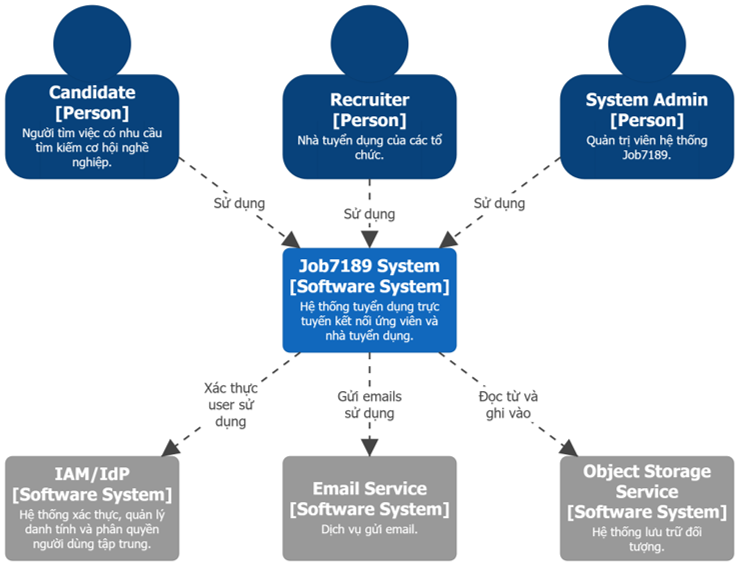
\includegraphics[width=0.88\textwidth]{images/context.png}
  \caption{Sơ đồ ngữ cảnh hệ thống Job7189}
  \label{fig:intro_context_job7189}
\end{figure}

\begin{figure}[H]
  \centering
  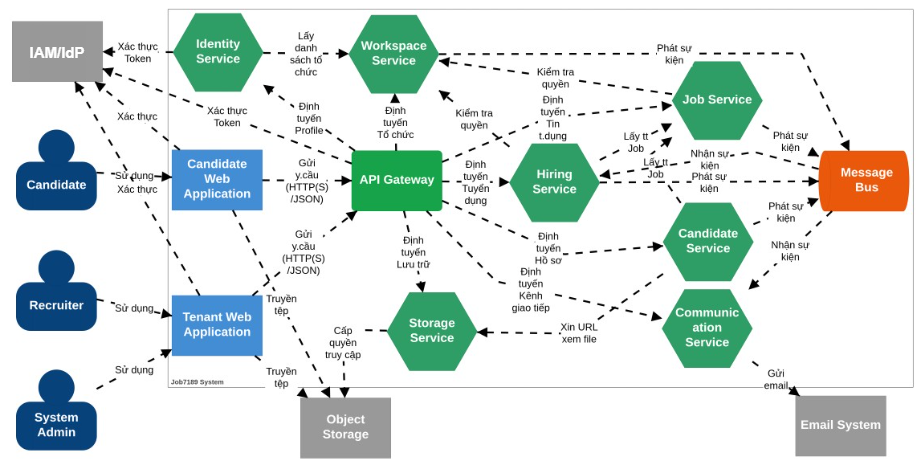
\includegraphics[width=0.92\textwidth]{images/container.png}
  \caption{Kiến trúc container của hệ thống Job7189 (góc nhìn nghiệp vụ)}
  \label{fig:intro_container_job7189}
\end{figure}

\begin{figure}[H]
  \centering
  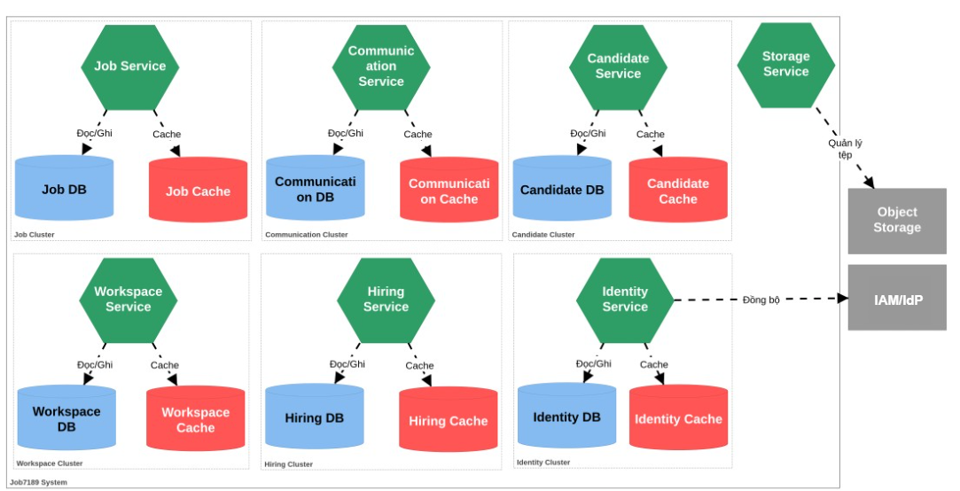
\includegraphics[width=0.92\textwidth]{images/containerdb.png}
  \caption{Kiến trúc container của hệ thống Job7189 (góc nhìn dữ liệu)}
  \label{fig:intro_containerdb_job7189}
\end{figure}

\textbf{Phạm vi thực nghiệm:} Đồ án tập trung hiện thực hóa kiến trúc Zero Trust ở phía máy chủ (Server-side) và khối lượng công việc (Workload). Các mục tiêu chính bao gồm: định danh thực thể, phân đoạn mạng vi mô, quản lý thông tin xác thực động và giám sát thời điểm chạy. 

\textbf{Loại trừ có chủ đích:} Việc kiểm tra tư thế bảo mật của thiết bị người dùng cuối (Client Device Posture) và các cơ chế đánh giá truy cập liên tục nâng cao tích hợp GitOps (CAEP/GitOps) nằm ngoài phạm vi của nguyên mẫu (PoC) này.

%==============================================================================
% 3.2 KHẢO SÁT HIỆN TRẠNG (DISCOVERY)
%==============================================================================
\section{Khảo sát hiện trạng hệ thống (Discovery)}

Tuân thủ nguyên tắc triển khai của tiêu chuẩn NIST SP 800-207 (Bước 1 đến Bước 3), trước khi áp dụng chính sách cưỡng chế, hệ thống cần trải qua giai đoạn khảo sát toàn diện. Kết quả khảo sát là đầu vào bắt buộc để xây dựng tập luật kiểm soát truy cập sát với thực tế.

\begin{itemize}[itemsep=6pt, parsep=0pt]
    \item \textbf{Kiểm kê chủ thể (Subjects):} Bao gồm người dùng cuối được quản lý qua Keycloak Realm \texttt{job7189}; quản trị viên hệ thống qua Realm \texttt{7189\_internal}; và các thực thể phi con người (7 vi dịch vụ, các tác vụ CronJob, bộ điều khiển PDP).
    
    \item \textbf{Kiểm kê tài sản (Assets):} Cụm thực nghiệm gồm 4 máy chủ (1 Control Plane, 3 Worker Nodes) kết nối qua mạng riêng ảo Tailscale. Tài sản phần mềm bao gồm 7 vi dịch vụ nghiệp vụ, 7 bản sao Redis, cụm MySQL và Kafka.
    
    \item \textbf{Bản đồ luồng dữ liệu (Data Flows):} Thay vì phỏng đoán luồng giao tiếp dựa trên mã nguồn, đồ án sử dụng công cụ Hubble chạy ở \textbf{chế độ ghi nhận (Audit mode)}. Cơ chế này cho phép bắt toàn bộ lưu lượng mạng thực tế sinh ra trong quá trình hệ thống hoạt động bình thường mà không làm rớt gói tin. Từ dữ liệu đo lường từ xa (telemetry) thu thập được, hệ thống vẽ ra bản đồ luồng dữ liệu chính xác gồm 3 trục: (1) Luồng Bắc-Nam từ API Gateway; (2) Luồng Đông-Tây giữa các vi dịch vụ; (3) Luồng truy xuất cơ sở dữ liệu. Đây là căn cứ kỹ thuật trực tiếp để định nghĩa các chính sách phân đoạn mạng vi mô ở giai đoạn sau.
\end{itemize}

%==============================================================================
% 3.3 THIẾT KẾ ZERO TRUST CHO JOB7189
%==============================================================================
\section{Thiết kế Zero Trust cho hệ thống job7189}

\subsection{Phân bổ không gian tên (Namespace)}

Nhằm thiết lập ranh giới cách ly logic ban đầu, khối lượng công việc được phân bổ vào 7 không gian tên độc lập dựa trên mức độ rủi ro và chức năng vận hành.

% [CHÈN C3 CŨ VÀO ĐÂY: Sơ đồ TikZ hoặc hình ảnh mô tả phân bổ Namespace (fig:c3_namespace_map)]

\subsection{Lộ trình triển khai 5 giai đoạn}

Quá trình cài đặt tuân theo lộ trình chuyển đổi đề xuất tại Mục 2.3.3 (bảy bước NIST SP 800-207, nguyên tắc 'audit trước $\rightarrow$ enforce sau'), được cụ thể hóa thành năm giai đoạn thực thi trên hệ thống \texttt{job7189}:

\begin{enumerate}[itemsep=6pt, parsep=0pt]
    \item \textbf{Giai đoạn 0 (Baseline hạ tầng):} Triển khai hạ tầng và ứng dụng cơ bản chưa có cơ chế Zero Trust.
    \item \textbf{Giai đoạn 1 (Quản lý tài nguyên \& định danh):} Cài đặt SPIRE, cert-manager và Keycloak để thiết lập gốc tin cậy.
    \item \textbf{Giai đoạn 2 (Chế độ Audit):} Triển khai các điểm thực thi (Cilium, Gatekeeper, Tetragon) ở chế độ ghi nhận, thu thập dữ liệu luồng.
    \item \textbf{Giai đoạn 3 (Mở rộng Cưỡng chế - Enforce):} Kích hoạt chính sách chặn mặc định, áp dụng luật mạng tường minh.
    \item \textbf{Giai đoạn 4 (Thích ứng):} Kích hoạt vòng lặp phản hồi của bộ điều khiển PDP và cấp phát bí mật động qua Vault.
\end{enumerate}

%==============================================================================
% 3.4 TRIỂN KHAI 5 THÀNH PHẦN CHỨC NĂNG
%==============================================================================
\section{Triển khai 5 thành phần chức năng}

Triển khai bám sát năm thành phần chức năng (TC1–TC5) đã đề xuất ở Chương 2. Trong đó, hệ thống quản lý bí mật (Vault) được trình bày với tư cách là Bộ điều phối chính sách thuộc TC3, không phải một thành phần tách rời.

% [CHÈN C3 CŨ VÀO ĐÂY: Sơ đồ fig:c3_5layer_design (Vẽ lại 5 hộp theo thứ tự luồng TC1->TC5, Vault chui vào TC3, Cosign vào TC2, PDP loop vào TC5)]

\subsection{TC1 — Định danh và Xác thực}
\begin{itemize}[itemsep=6pt, parsep=0pt]
    \item \textbf{Công nghệ:} Keycloak (Người dùng) và SPIRE (Workload).
    \item \textbf{Cấu hình:} SPIRE Server lưu trữ gốc tin cậy. SPIRE Agent trên mỗi Node thực hiện chứng thực khối lượng công việc, cấp phát chứng chỉ X.509 SVID với thời gian sống ngắn.
    \item \textbf{Chế độ lỗi:} Nếu SPIRE Server gián đoạn, các SVID hiện tại vẫn hợp lệ cho đến khi hết hạn. Workload mới không thể khởi động khi chưa có SVID hợp lệ — đây là hành vi từ chối an toàn có chủ đích.
\end{itemize}

\subsection{TC2 — Đánh giá tư thế và tình báo đe dọa}
\begin{itemize}[itemsep=6pt, parsep=0pt]
    \item \textbf{Công nghệ:} Trivy Operator, Sigstore (Cosign), và FireHOL.
    \item \textbf{Cấu hình:} Trivy liên tục quét lỗ hổng sinh ra \texttt{VulnerabilityReport}. Tại cổng nạp (Admission), Sigstore policy-controller kiểm tra tính hợp lệ của chữ ký image. Trong phạm vi PoC, cơ chế này đang hoạt động ở chế độ cảnh báo (\texttt{mode=warn}). Danh sách IP độc hại từ FireHOL được đồng bộ vào \texttt{CiliumCIDRGroup}.
\end{itemize}

\subsection{TC3 — Ra quyết định (PE + PA + Vault)}
\begin{itemize}[itemsep=6pt, parsep=0pt]
    \item \textbf{Công nghệ:} Bộ điều khiển PDP (Python/Kopf) và HashiCorp Vault.
    \item \textbf{Cấu hình:} PDP Controller đóng vai trò Động cơ chính sách (PE), liên tục đọc dữ liệu từ TC2 và TC5 để tính toán mức độ rủi ro, gán nhãn \texttt{score-bucket} cho Pod. Vault đóng vai trò Bộ điều phối (PA), tiếp nhận định danh JWT-SVID của Pod để ra quyết định cấp phát thông tin xác thực cơ sở dữ liệu động (JIT).
\end{itemize}

\subsection{TC4 — Thực thi chính sách đa tầng}
\begin{itemize}[itemsep=6pt, parsep=0pt]
    \item \textbf{Công nghệ:} Kong Gateway, Cilium eBPF, OPA Gatekeeper, Tetragon.
    \item \textbf{Cấu hình:} Kong kiểm tra JWT tại biên. Cilium thực thi chính sách mạng nội bộ dựa trên nhãn định danh. OPA Gatekeeper chặn các cấu hình sai lệch. Tetragon can thiệp trực tiếp tại Kernel. Động tác tiêm mật khẩu động vào Pod được thực hiện bởi Vault Agent sidecar (mount vào \texttt{tmpfs}).
\end{itemize}

\subsection{TC5 — Quan sát và Phản hồi}
\begin{itemize}[itemsep=6pt, parsep=0pt]
    \item \textbf{Công nghệ:} EFK Stack, Prometheus, Hubble.
    \item \textbf{Cấu hình:} Hubble ánh xạ gói tin mạng với định danh thực thể. Toàn bộ sự kiện an ninh được đẩy về Elasticsearch. Dữ liệu này đóng vòng phản hồi về TC3 để hệ thống tự động điều chỉnh chính sách cưỡng chế.
\end{itemize}

%==============================================================================
% 3.5 KIỂM CHỨNG THỰC NGHIỆM
%==============================================================================
\section{Kiểm chứng thực nghiệm các kịch bản tấn công}

% [CHÈN C3 CŨ VÀO ĐÂY: Dán toàn bộ Kịch bản 1 đến Kịch bản 6 của bạn vào đây. Giữ đúng thứ tự KB1 = Tetragon, KB2 = Vault... kèm theo các block code/log thực tế. Nhớ bổ sung log Exit Code 137 cho Tetragon như đã thống nhất.]

%==============================================================================
% 3.6 ĐÁNH GIÁ TỔNG HỢP VÀ HẠN CHẾ
%==============================================================================
\section{Đánh giá tổng hợp và hạn chế}

Đồ án kiểm chứng 6 kịch bản tấn công-phòng thủ toàn trình (KB1–KB6) với nhật ký thực tế, bao phủ 10 kỹ thuật MITRE ATT\&CK for Containers. Bảng \ref{tab:c3_mitre_summary} liệt kê tổng hợp 17 kỹ thuật tấn công, bao gồm 10 kỹ thuật đã kiểm chứng thực tế và 7 kỹ thuật ở mức độ định hướng thiết kế, nhằm đánh giá độ phủ phòng thủ toàn diện của kiến trúc chứ không chỉ giới hạn ở phần đã chạy.

% [CHÈN C3 CŨ VÀO ĐÂY: Dán Bảng 17 dòng MITRE vào đây. Nhớ có cột 'Mức minh chứng' (Đã kiểm chứng [A] / Một phần / Thiết kế)]

\subsection{Mức độ cưỡng chế thực tế của hệ thống}

Để đảm bảo tính trung thực khoa học, Bảng \ref{tab:enforcement_level} đối chiếu trạng thái cấu hình thực tế của cụm thực nghiệm (tính đến thời điểm báo cáo) so với lý thuyết thiết kế. Trong phạm vi PoC, một số cơ chế (như Gatekeeper, Cosign) hoạt động ở chế độ ghi nhận (monitor mode) theo đúng bước 6 của lộ trình NIST SP 800-207 nhằm tránh gián đoạn dịch vụ hợp lệ.

\begin{table}[H]
\centering
\caption{Mức độ cưỡng chế thực tế của các cơ chế bảo mật}
\label{tab:enforcement_level}
\renewcommand{\arraystretch}{1.3}
\begin{tabularx}{\textwidth}{|p{3.5cm}|X|X|}
\hline
\textbf{Cơ chế / Công cụ} & \textbf{Trạng thái thực tế trên cụm} & \textbf{Ghi nhận trong báo cáo} \\
\hline
mTLS (Cilium) & \texttt{mesh-auth-enabled=true} (Dùng SVID) & Đã bật. \\
\hline
Mã hóa L3 (WireGuard) & \texttt{enable-wireguard=false} & Bắt buộc tắt để tránh xung đột mã hóa kép do Tailscale đã đảm nhận L3. \\
\hline
Giám sát Runtime (Tetragon) & v1.7.0, \texttt{Sigkill enforce} ở 4 namespace (có TracingPolicy). & Ngắt tại nhân, với TracingPolicy tương ứng. \\
\hline
Chữ ký số (Cosign) & 3 ClusterImagePolicy đang ở \texttt{mode=warn}. & WARN — chuyển enforce ở giai đoạn sau. Chốt cứng dựa vào digest-pin. \\
\hline
Kiểm soát cổng nạp (Gatekeeper) & Hoạt động ở chế độ \texttt{dryrun} (Audit), chỉ \texttt{zta-block-host-mounts = deny}. & Phần lớn audit; chốt cứng là digest-pin + netpol + seccomp. \\
\hline
Trivy Operator & Đang chạy, $\sim$5 VulnerabilityReport. & Posture feed hoạt động. \\
\hline
Threat-Intel & CIDRGroup $\sim$2000 CIDR, CronJob active. & Đã đồng bộ. \\
\hline
Vòng lặp PDP & Thành phần đủ, chưa demo e2e (mọi pod đang ở mức high). & Đã hiện thực một phần — cần pod điểm thấp để minh chứng. \\
\hline
\end{tabularx}
\end{table}

\subsection{Hạn chế của nguyên mẫu thực nghiệm}

Mô hình điểm tin cậy và vòng lặp phản hồi PDP hiện tại đã được triển khai thành phần điều khiển (controller), tuy nhiên chưa được kiểm chứng tự động toàn trình (end-to-end) do mọi khối lượng công việc hiện tại đều đạt điểm tin cậy cao. Việc minh chứng kịch bản cô lập tự động đòi hỏi phải chủ động tiêm một vùng chứa mang lỗ hổng nghiêm trọng vào hệ thống.

Bên cạnh đó, trục đánh giá \textit{Phân cấp dịch vụ (Service Tier)} đã được đọc từ nhãn của Kubernetes nhưng chưa được tích hợp vào hàm tính điểm. Trục \textit{Khả năng khai thác (Exploitability)} hiện đang dừng ở mức định hướng thiết kế, do báo cáo của Trivy Operator chưa hỗ trợ trực tiếp thông tin về mã khai thác công khai, đòi hỏi hệ thống phải tích hợp thêm nguồn cấp dữ liệu từ CISA KEV hoặc EPSS trong tương lai.
% !TEX encoding = UTF-8
\chapter{Thử nghiệm và Đánh giá}

\section{Mục tiêu chương}

Chương này trình bày kế hoạch thử nghiệm và khung đánh giá cho giai đoạn tiếp theo của đồ án, nhằm kiểm chứng mức độ hiệu quả của kiến trúc Zero Trust đã triển khai trên hệ thống JOB7189. Trọng tâm là chứng minh mối liên hệ giữa từng cơ chế kiểm soát và các nguyên lý (tenets) trong NIST SP 800-207 \cite{nist800207}.

\section{Kịch bản thử nghiệm}

Mỗi kịch bản được thiết kế để xác thực một nhóm nguyên lý cụ thể của NIST SP 800-207.

\subsection{Kịch bản 1: Lateral Movement}

\textbf{Mục tiêu:} Pod bị chiếm quyền cố gắng truy cập dịch vụ ngoài chính sách cho phép.

\textbf{Ý nghĩa kiểm chứng:}
\begin{itemize}
    \item Least Privilege (đặc quyền tối thiểu).
    \item Micro-segmentation với nguyên tắc Deny-All, Allow-Explicit.
\end{itemize}

\subsection{Kịch bản 2: API Abuse}

\textbf{Mục tiêu:} Gọi sai endpoint hoặc sai HTTP method và bị Cilium L7 policy chặn.

\textbf{Ý nghĩa kiểm chứng:}
\begin{itemize}
    \item Per-request Access Decision (quyết định truy cập theo từng yêu cầu).
\end{itemize}

\subsection{Kịch bản 3: Runtime Anomaly}

\textbf{Mục tiêu:} Phát sinh hành vi bất thường trong Pod (ví dụ thực thi lệnh hệ thống trái phép).

\textbf{Ý nghĩa kiểm chứng:}
\begin{itemize}
    \item Continuous Monitoring (giám sát liên tục).
\end{itemize}

\textit{Lưu ý:} Kịch bản này sẽ được hoàn thiện khi lớp Runtime Enforcement (Tetragon) được triển khai đầy đủ (bổ sung sau).

\subsection{Kịch bản 4: Credential Reuse}

\textbf{Mục tiêu:} Vault credential hết hạn TTL, bị thu hồi, và kiểm tra khả năng chống tái sử dụng thông tin xác thực cũ.

\textbf{Ý nghĩa kiểm chứng:}
\begin{itemize}
    \item Dynamic Trust Evaluation (đánh giá tin cậy động theo thời gian).
\end{itemize}

\section{Phân tích kết quả}

Khung phân tích kết quả dự kiến gồm ba lớp:
\begin{itemize}
    \item \textbf{Định lượng giảm attack surface:} so sánh số attack path khả thi trước và sau khi áp dụng ZTA.
    \item \textbf{Đánh giá blast radius:} đo số dịch vụ mà một Pod bị compromise có thể reach trước và sau policy.
    \item \textbf{Đối chiếu Traceability Matrix:} ánh xạ theo chuỗi \textit{threat $\rightarrow$ control $\rightarrow$ result} để chứng minh tính giải thích được của từng kết quả thử nghiệm.
\end{itemize}

\section{Đánh giá hiệu năng}

Nội dung đánh giá hiệu năng tập trung vào các chỉ số trọng yếu:
\begin{itemize}
    \item \textbf{Latency P99:} so sánh trước/sau khi áp dụng Network Policy và mTLS.
    \item \textbf{Resource overhead:} mức tiêu thụ tài nguyên của Cilium, Tetragon, Vault Agent.
    \item \textbf{Trade-off bảo mật - hiệu năng:} phân tích mức tăng độ trễ và tài nguyên đổi lấy mức giảm rủi ro bảo mật.
\end{itemize}

\section{Đánh giá mức độ tuân thủ NIST SP 800-207}

Khung tuân thủ sẽ được tổng hợp theo ba nội dung:
\begin{itemize}
    \item \textbf{Bảng đối chiếu 7 Tenets:} ánh xạ từng nguyên lý của NIST SP 800-207 với các cơ chế đã triển khai trong hệ thống.
    \item \textbf{Known Limitations:} ghi nhận minh bạch các giới hạn hiện tại như Kafka plaintext, shared physical DB, HMAC shared key.
    \item \textbf{Kết luận xác thực học thuật:} đánh giá mức độ mà khung lý thuyết ở Chương 2 được kiểm chứng qua case study JOB7189.
\end{itemize}

\section{Thảo luận}

Phần thảo luận tập trung vào ba hướng:
\begin{itemize}
    \item \textbf{Tính tổng quát của khung đề xuất:} khả năng áp dụng cho các hệ Microservices ngoài JOB7189.
    \item \textbf{Khả năng mở rộng trong production:} điều kiện để chuyển từ PoC sang vận hành thực tế.
    \item \textbf{Hướng phát triển tiếp theo:} SPIFFE per-workload certificate, Kafka SASL/SSL, physical DB separation.
\end{itemize}

% !TEX encoding = UTF-8

\chapter*{Kết luận}
\addcontentsline{toc}{chapter}{Kết luận}

Đồ án \textbf{``Nghiên cứu Kiến trúc Zero Trust và Ứng dụng trong Bảo mật Hệ thống Microservices trên Kubernetes''} tập trung vào ba việc: hệ thống hóa nền tảng Zero Trust, đề xuất kiến trúc bảo vệ phù hợp với Kubernetes và thử nghiệm kiến trúc đó trên hệ thống Job7189.

\paragraph{Về mặt lý thuyết:}
\begin{itemize}
    \item Hệ thống hóa các nguyên lý Zero Trust và kiến trúc tham chiếu theo \textbf{NIST SP 800-207}~\parencite{nist800207,kindervag2010build,gilman2017zero}, gồm mô hình ra quyết định, điểm thực thi chính sách và các nguồn dữ liệu phục vụ đánh giá truy cập.
    \item Phân tích các rủi ro đặc thù của vi dịch vụ trên Kubernetes, gồm lưu lượng nội bộ lớn, vòng đời ngắn của thực thể chạy, quản lý bí mật phân tán, rủi ro hạ tầng dùng chung và nguy cơ từ chuỗi cung ứng phần mềm~\parencite{nist800204_microservices,rice2019kubernetes,machine_identity_report}.
    \item Đề xuất khung kiến trúc Zero Trust gồm năm thành phần chức năng, triển khai mô hình tham chiếu của NIST bằng các công cụ mã nguồn mở phù hợp với Kubernetes~\parencite{nist800207,kubernetes_docs,cisa_ztmm2023}.
    \item Xây dựng mô hình đe dọa dựa trên MITRE ATT\&CK cho Kubernetes~\parencite{mitre_containers,owasp_api2023}, qua đó xác định các kịch bản tấn công và cơ chế phòng thủ tương ứng.
\end{itemize}

\paragraph{Về mặt thực nghiệm trên hệ thống Job7189:}
\begin{itemize}
    \item Triển khai phân đoạn mạng vi mô bằng CiliumNetworkPolicy~\parencite{cilium_docs,ebpf_io}: áp dụng chính sách từ chối mặc định cho các không gian tên trọng yếu, sau đó chỉ mở các luồng cần thiết giữa dịch vụ, CSDL, bộ nhớ đệm và thành phần hạ tầng.
    \item Hiện thực hóa quản lý bí mật động bằng HashiCorp Vault~\parencite{vault_docs}: bảy vi dịch vụ nhận thông tin kết nối CSDL ngắn hạn, được ghi vào bộ nhớ tạm của pod và tự xoay vòng mà không làm gián đoạn ứng dụng~\parencite{nist800207,machine_identity_report}.
    \item Xây dựng cơ chế xác thực tập trung với Keycloak~\parencite{keycloak_docs} và Kong Gateway~\parencite{kong_docs}; các yêu cầu đi vào hệ thống được kiểm tra JWT theo chữ ký RS256 trước khi chuyển tới dịch vụ nghiệp vụ~\parencite{rfc7519_jwt,oidc_core,rfc6749_oauth2}.
    \item Thiết lập lớp quan sát gồm EFK, Prometheus, Grafana và Hubble~\parencite{elk_docs,prometheus_docs,grafana_docs,hubble_docs}; dữ liệu thu được hỗ trợ kiểm toán, quan sát luồng mạng và đối chiếu kết quả của các chính sách an ninh.
    \item Kiểm chứng 11 kịch bản an ninh theo hướng phân biệt rõ giữa chặn chủ động, ghi nhận, giảm thiểu tác động và khôi phục thủ công. Kết quả cho thấy hệ thống có thể chặn hoặc kiểm soát nhiều hành vi như quét mạng nội bộ, gọi API sai quyền, truy cập CSDL trái phép, chạy công cụ mạng bị cấm, triển khai container image chưa được phê duyệt và gửi dữ liệu ra bên ngoài trái chính sách.
\end{itemize}

\paragraph{Hạn chế và hướng phát triển:}
Hệ thống Job7189 trong đồ án được dùng như một môi trường mô phỏng trên cụm \texttt{kubeadm} nhiều nút kết nối qua Tailscale~\parencite{kubeadm_docs,tailscale_docs}; mục tiêu là tạo đủ luồng nghiệp vụ và luồng hạ tầng để thử các cơ chế bảo vệ, chưa phải một triển khai Zero Trust hoàn chỉnh cho môi trường sản xuất. Các hạn chế chính gồm:
\begin{itemize}
    \item Cơ chế tự động phản hồi chưa được kiểm chứng toàn trình. Bộ điều khiển chính sách đã có vai trò tính toán và gán nhãn rủi ro, nhưng kịch bản cô lập tự động khi điểm rủi ro giảm vẫn cần dữ liệu thử nghiệm sát thực tế hơn.
    \item Việc đánh giá thiết bị người dùng nằm ngoài phạm vi đồ án. Hệ thống mới tập trung vào thực thể chạy trong cụm Kubernetes, trong khi NIST SP 800-207 còn yêu cầu đánh giá liên tục trạng thái thiết bị truy cập~\parencite{nist800207,cisa_ztmm2023}.
    \item Hệ thống chưa có cơ chế thu hồi phiên tự động khi phát hiện bất thường sau thời điểm cấp token. Đây là khoảng trống liên quan đến đánh giá truy cập liên tục và cần được bổ sung bằng luồng cảnh báo, đánh giá rủi ro và thu hồi phiên~\parencite{openid_caep,microsoft_aitm}.
    \item Việc thu hồi bí mật động hiện chủ yếu dựa vào thời gian sống và vòng xoay lease; Vault chưa tự thu hồi ngay theo tín hiệu runtime từ Tetragon. Tương tự, khôi phục chính sách mạng khi bị sửa hoặc xóa vẫn cần thao tác vận hành, chưa có bộ điều khiển tự phục hồi liên tục.
    \item Một số cơ chế vẫn vận hành ở chế độ ghi nhận hoặc cảnh báo để tránh gián đoạn dịch vụ trong phòng thí nghiệm, chẳng hạn một phần kiểm soát khi tiếp nhận tài nguyên Kubernetes và kiểm chứng chữ ký container image. Khi đưa vào môi trường nghiêm ngặt hơn, cần chuyển dần sang chế độ cưỡng chế sau khi đã đủ dữ liệu quan sát.
    \item Cấu hình Vault hiện còn phụ thuộc vào thành phần hỗ trợ trong môi trường thử nghiệm. Khi triển khai thật, cần thay bằng cơ chế lưu trữ và tự mở khóa bền vững hơn, chẳng hạn Raft storage với PersistentVolume hoặc dịch vụ quản lý khóa phù hợp~\parencite{vault_docs}.
\end{itemize}

Kết quả quan trọng nhất của đồ án không phải là một hệ thống đã sẵn sàng đưa vào sản xuất, mà là một mô hình triển khai có thể quan sát và kiểm chứng được. Trên cùng một cụm Kubernetes, các lớp định danh, phân đoạn mạng, kiểm soát truy cập, bí mật động và quan sát đã phối hợp được với nhau. Đây là nền tảng để tiếp tục hoàn thiện các phần còn thiếu: phản hồi tự động, đánh giá rủi ro liên tục và chuyển dần các cơ chế cảnh báo sang cưỡng chế.


% PHẦN CUỐI (BACK MATTER)
%---------------------------------------------------
\clearpage
\pagestyle{plain} 

\printbibliography
 
\end{document}